\documentclass[12pt,a4paper]{article}

\usepackage[brazil]{babel}
\usepackage[utf8]{inputenc}
\usepackage[T1]{fontenc}
\usepackage{lmodern}
\usepackage[margin=2.5cm]{geometry}
\usepackage{amsmath,amssymb}
\usepackage{graphicx}
\usepackage{booktabs}
\usepackage{multirow}
\usepackage{float}
\usepackage[font=small,labelfont=bf]{caption}
\usepackage[table]{xcolor}
\usepackage{hyperref}
\usepackage{url}
\def\UrlBreaks{\do\_\do/\do.}
\urlstyle{tt}
\emergencystretch=2em

\hypersetup{colorlinks=true, linkcolor=blue!50!black, urlcolor=blue!50!black, citecolor=blue!50!black}
\graphicspath{{figuras/}}
\newcommand{\bom}[1]{\textbf{#1}}
\newcommand{\ruim}[1]{\textcolor{red!70!black}{#1}}

\title{Poda de Camadas em Modelos Fundacionais para Grafos\\
\large Relatório de Resultados}
\author{}
\date{\today}

\begin{document}

\maketitle
\tableofcontents
\newpage

\section{Introdução}

Modelos fundacionais para grafos (\emph{Graph Foundation Models}, GFMs) são pré-treinados uma vez e aplicados a grafos novos sem re-treino (zero-shot) ou com poucos exemplos rotulados (aprendizado em contexto). Esses modelos são grandes para o tamanho dos grafos em que costumam ser usados, e não se sabe quanto da sua profundidade é de fato necessária. Em modelos de linguagem, o ShortGPT~\cite{shortgpt} mostrou que muitas camadas mudam pouco a representação e podem ser removidas inteiras, escolhidas por uma métrica simples, o \emph{Block Influence} (BI).

Este trabalho pergunta se o mesmo vale para GFMs:
\begin{enumerate}
  \item \textbf{O BI encontra camadas redundantes?} Isto é, a ordem de poda pelo BI é melhor que uma ordem aleatória e se aproxima de uma ordem de referência escolhida com rótulos (ablação)?
  \item \textbf{Quanto se pode podar sem re-treino?} Curva de desempenho retido em função do número de camadas removidas, e quanto isso economiza em parâmetros, tempo e memória.
  \item \textbf{A destilação de conhecimento (KD) recupera o modelo podado?} E começar do modelo podado é melhor do que treinar um student da mesma arquitetura a partir de pesos aleatórios?
\end{enumerate}

Foram estudados seis modelos com arquiteturas e formas de uso diferentes: AnyGraph~\cite{anygraph} e OpenGraph~\cite{opengraph} (zero-shot), Prodigy~\cite{prodigy} (\emph{few-shot} por grafo de tarefa) e três \emph{prior-data fitted networks} (PFNs) de aprendizado em contexto: GraphPFN~\cite{graphpfn}, G2T-FM~\cite{g2tfm} e NodePFN~\cite{nodepfn}. A recuperação após a poda usa destilação de conhecimento~\cite{hinton-kd}. OpenGraph e Prodigy foram avaliados por João Victor e aparecem aqui de forma resumida. Para que os resultados sejam comparáveis entre modelos, os PFNs usam o mesmo protocolo (datasets e splits do artigo do GraphPFN, mesmas ordens de poda, mesma normalização pelo acaso e mesmo protocolo de KD), e o AnyGraph usa a versão desse protocolo que cabe num modelo zero-shot (Seção~\ref{sec:any-fases}). A Seção~\ref{sec:sintese} reúne os modelos lado a lado.

Todos os experimentos rodaram numa única GPU de 16\,GB (RTX 5060 Ti) com 31\,GB de RAM. As adaptações que isso exigiu estão descritas em cada seção e reunidas na Seção~\ref{sec:limitacoes}.

%==============================================================================
\section{AnyGraph}
%==============================================================================

Esta seção avalia se o AnyGraph tem camadas redundantes, isto é, se removê-las não piora (ou piora pouco) o modelo. As camadas são escolhidas pelo \emph{Block Influence} (BI), medido no modelo inteiro.

\subsection{O modelo}

O AnyGraph é um \emph{Mixture-of-Experts} com 8 experts. Cada expert é uma MLP de 8 camadas densas de 512 dimensões, com conexão residual e LayerNorm. Foram usados os dois checkpoints públicos, \path{pretrain_link1} e \path{pretrain_link2} (16,88\,M parâmetros cada). O teste oficial de classificação de nós do artigo usa o \path{pretrain_link2}.

\subsection{Metodologia}

\begin{itemize}
  \item \textbf{BI:} medido sobre a entrada real dos experts (saída dos projetores), propagando cada camada como no \texttt{forward} do modelo (densa, residual, LayerNorm). Foram usados 1\,500 nós amostrados do cora e do pubmed e 1\,500 vetores gaussianos de 512 dimensões (semente 42). Foram testadas as duas formas: cosseno, $1-\cos(h_{in},h_{out})$, e angular, $\arccos(\cos)/\pi$.
  \item \textbf{Poda:} as mesmas camadas são removidas em todos os experts. Tier 1 remove as 2 camadas de menor BI (5 e 6; $-25\%$ dos parâmetros, 12,66\,M); Tier 2 remove as 4 de menor BI (4, 5, 6 e 7; $-50\%$, 8,44\,M).
  \item \textbf{Avaliação:} zero-shot nos 5 datasets de classificação de nós do AnyGraph (arxiv, cora, home, pubmed e tech), com as configurações oficiais (\texttt{shot=0}, \texttt{gnn\_layer=3}, \texttt{latdim=512}). Métricas: acurácia e F1-macro, e o OVERALL é a média ponderada pelo número de nós de teste.
  \item \textbf{Repetições pareadas:} cada avaliação sorteia projetores novos (SVD aleatorizado), e só isso faz o modelo inteiro variar de 0,620 a 0,694 de acurácia. Por isso a avaliação foi refeita com 10 repetições. Em cada repetição, os projetores e a atribuição de expert usam a mesma semente para o modelo inteiro e para os podados, e a diferença podado $-$ inteiro tem intervalo de confiança de 95\% (t de Student, 9 g.l.).
\end{itemize}

\subsection{Resultados}

\subsubsection{Block Influence}

\begin{table}[H]
\centering
\caption{BI cosseno médio por camada (média dos 8 experts), cora. Em negrito, as 4 camadas de menor BI.}
\label{tab:any-bi}
\begin{tabular}{@{}lcccccccc@{}}
\toprule
Modelo & L0 & L1 & L2 & L3 & L4 & L5 & L6 & L7 \\
\midrule
link1 & ,078 & ,077 & ,153 & ,096 & \bom{,022} & \bom{,008} & \bom{,006} & \bom{,020} \\
link2 & ,106 & ,093 & ,161 & ,094 & \bom{,024} & \bom{,010} & \bom{,008} & \bom{,030} \\
\bottomrule
\end{tabular}
\end{table}

\begin{figure}[H]
\centering
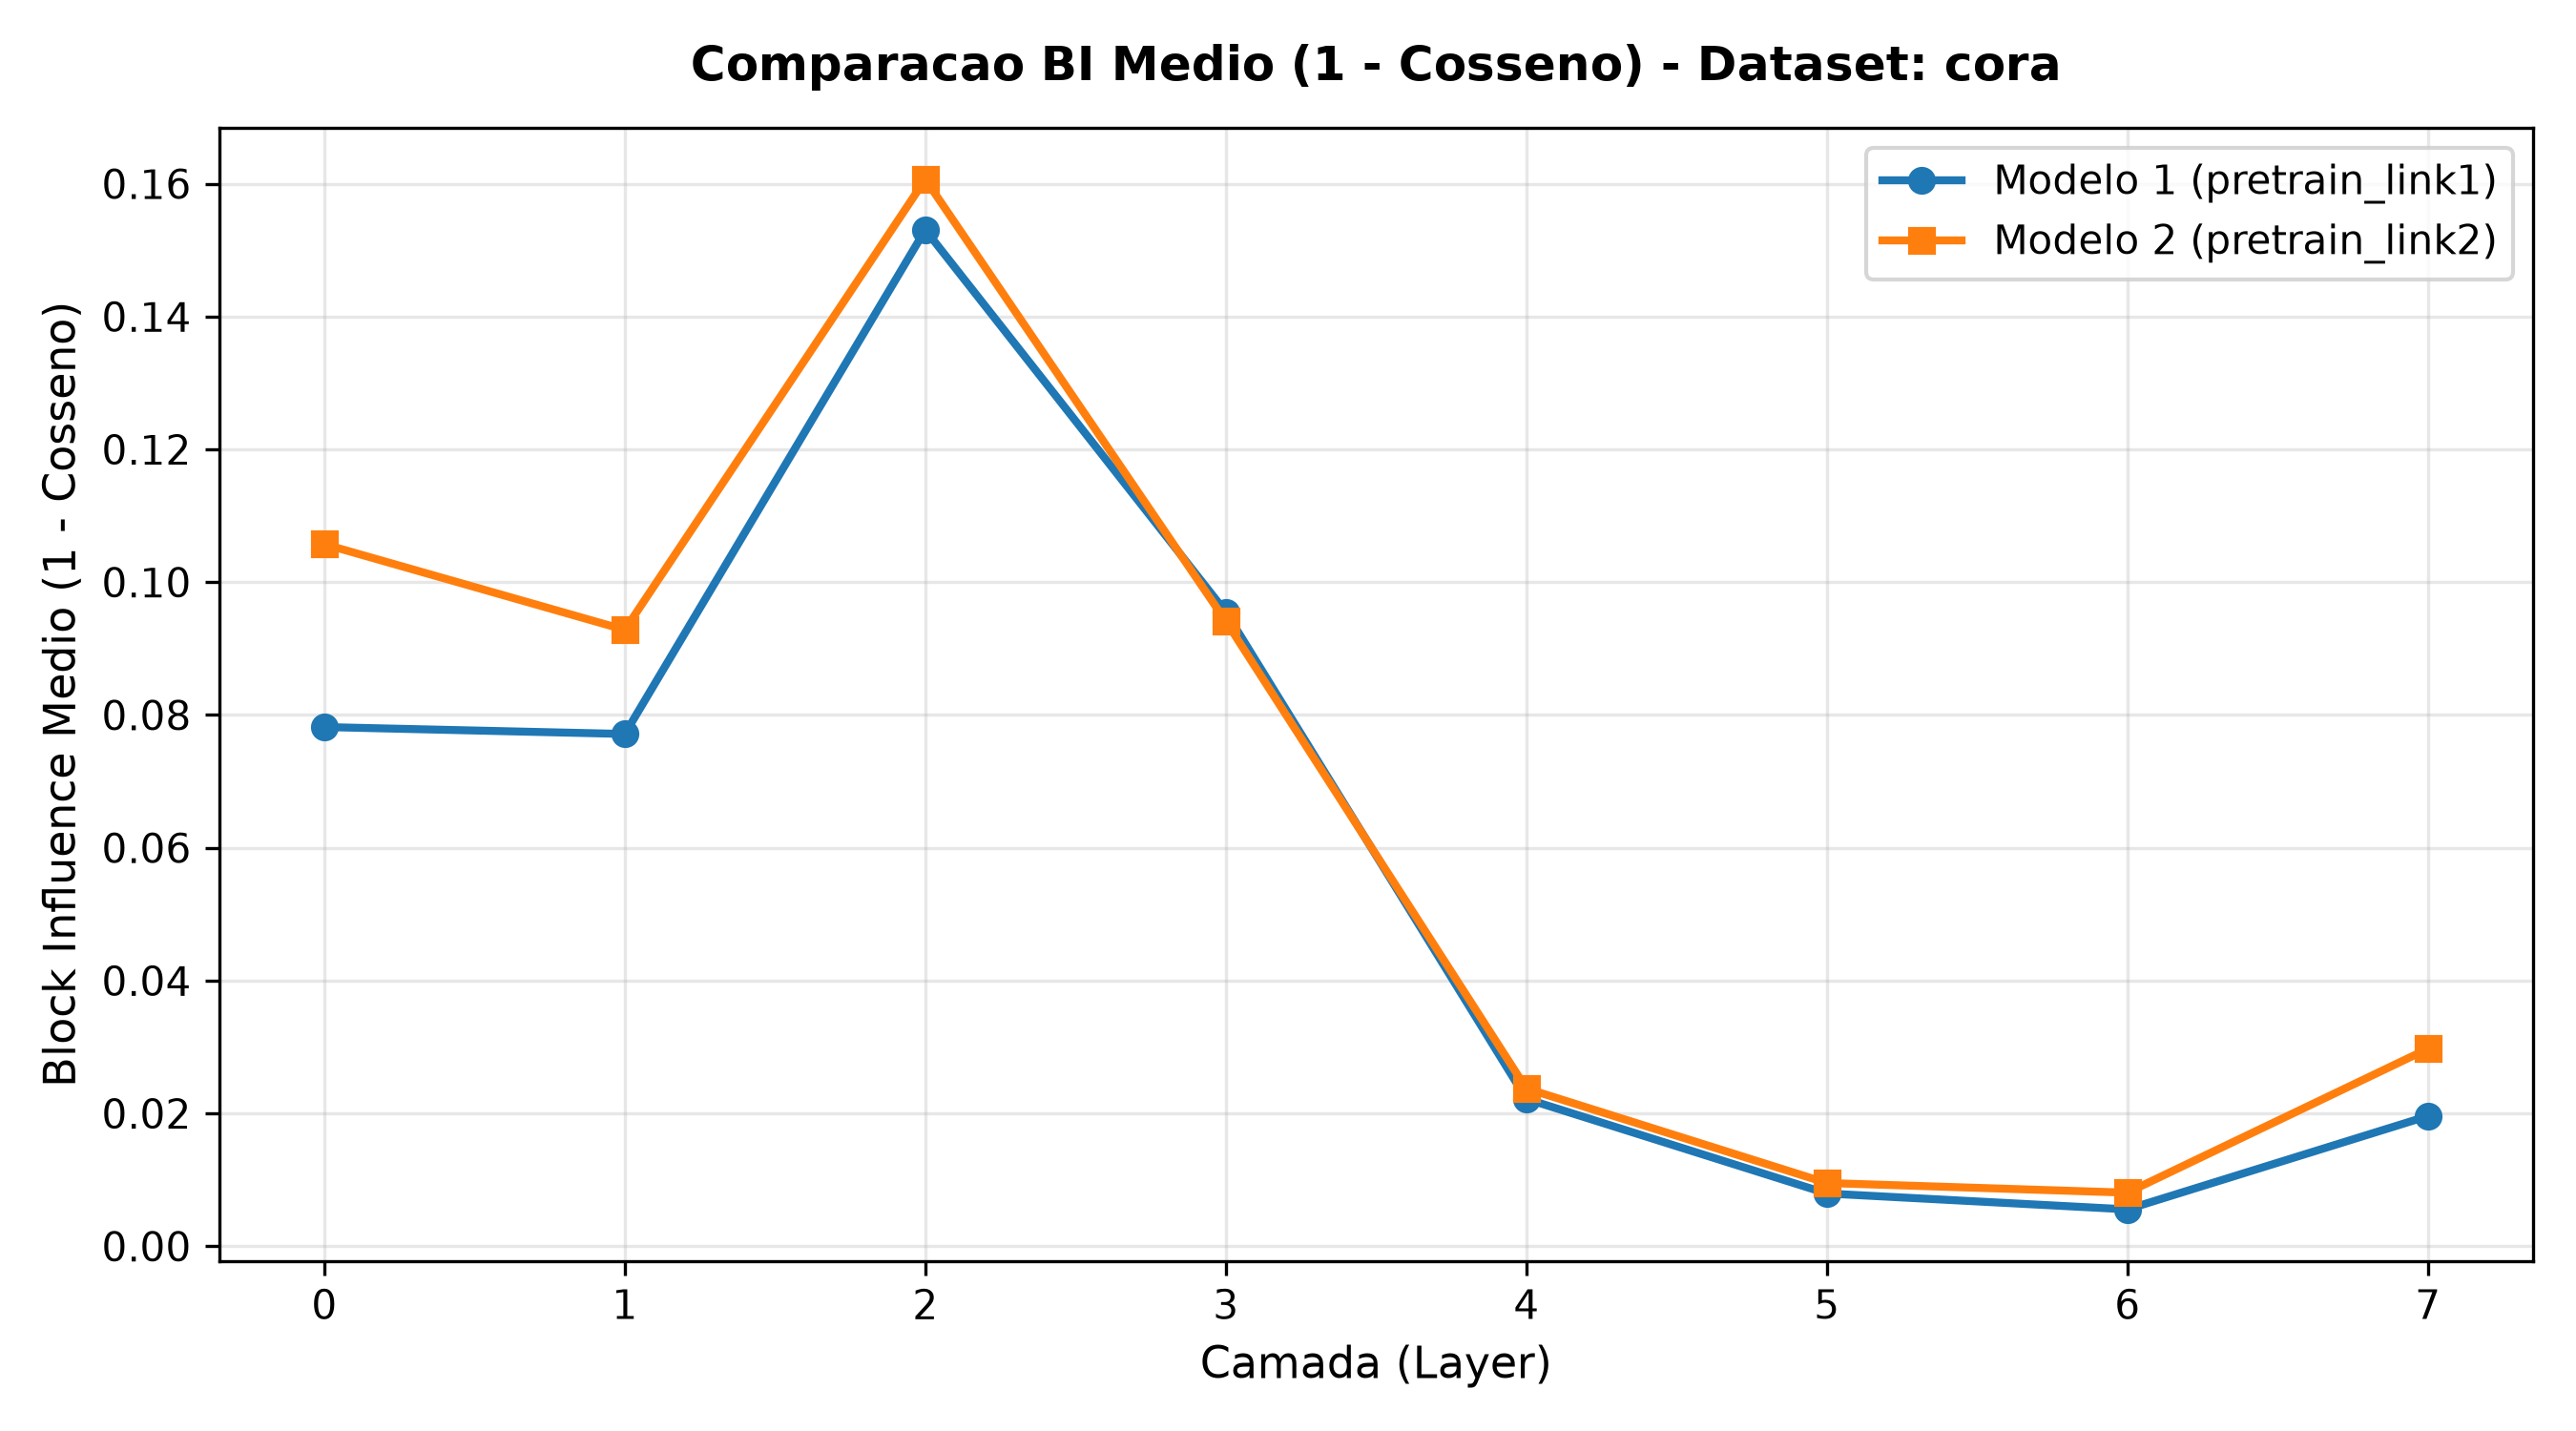
\includegraphics[width=0.8\textwidth]{anygraph/bi_por_camada_cora.png}
\caption{BI cosseno médio por camada no cora, nos dois checkpoints.}
\label{fig:any-bi}
\end{figure}

As camadas finais mudam pouco a representação: a ordem de poda é 6, 5, 7, 4 nos dois modelos. As camadas 4--7 são as 4 de menor BI em todos os 8 experts, e cosseno e angular dão rankings idênticos nos 6 casos (2 modelos $\times$ 3 conjuntos de dados). Por isso a poda usa só o cosseno.

\subsubsection{Poda}

\begin{table}[H]
\centering
\caption{OVERALL no teste, média $\pm$ desvio-padrão de 10 repetições, e diferença pareada podado $-$ inteiro com IC 95\%.}
\label{tab:any-poda}
\resizebox{\textwidth}{!}{%
\begin{tabular}{@{}llcccc@{}}
\toprule
Modelo & Configuração & Acurácia & F1 & $\Delta$ acurácia [IC 95\%] & $\Delta$ F1 [IC 95\%] \\
\midrule
link2 & Inteiro           & 0,663 $\pm$ 0,009 & 0,466 $\pm$ 0,008 & --- & --- \\
link2 & Tier 1 ($-25\%$)  & 0,690 $\pm$ 0,015 & 0,534 $\pm$ 0,014 & \bom{$+0{,}026$} [$+0{,}018$; $+0{,}035$] & \bom{$+0{,}068$} [$+0{,}053$; $+0{,}082$] \\
link2 & Tier 2 ($-50\%$)  & 0,577 $\pm$ 0,045 & 0,433 $\pm$ 0,027 & \ruim{$-0{,}087$} [$-0{,}116$; $-0{,}057$] & \ruim{$-0{,}033$} [$-0{,}055$; $-0{,}011$] \\
\midrule
link1 & Inteiro           & 0,572 $\pm$ 0,023 & 0,410 $\pm$ 0,026 & --- & --- \\
link1 & Tier 1 ($-25\%$)  & 0,575 $\pm$ 0,011 & 0,421 $\pm$ 0,010 & $+0{,}003$ [$-0{,}010$; $+0{,}016$] & $+0{,}011$ [$-0{,}004$; $+0{,}027$] \\
link1 & Tier 2 ($-50\%$)  & 0,639 $\pm$ 0,027 & 0,489 $\pm$ 0,030 & \bom{$+0{,}067$} [$+0{,}041$; $+0{,}094$] & \bom{$+0{,}079$} [$+0{,}047$; $+0{,}110$] \\
\bottomrule
\end{tabular}}
\end{table}

\begin{table}[H]
\centering
\caption{$\Delta$ acurácia (podado $-$ inteiro) por dataset. * = IC 95\% não cruza o zero.}
\label{tab:any-poda-ds}
\begin{tabular}{@{}llccccc@{}}
\toprule
Modelo & Configuração & arxiv & cora & home & pubmed & tech \\
\midrule
link2 & Tier 1 & $+0{,}025$* & $+0{,}004$* & $-0{,}015$ & $+0{,}031$* & $+0{,}047$* \\
link2 & Tier 2 & \ruim{$-0{,}111$*} & \ruim{$-0{,}087$*} & $+0{,}020$ & $-0{,}015$ & $-0{,}016$ \\
link1 & Tier 1 & $+0{,}004$ & \ruim{$-0{,}045$*} & $+0{,}036$* & $-0{,}022$ & $+0{,}023$ \\
link1 & Tier 2 & $+0{,}094$* & \ruim{$-0{,}027$*} & $-0{,}009$ & $+0{,}036$ & $-0{,}008$ \\
\bottomrule
\end{tabular}
\end{table}

\begin{itemize}
  \item \textbf{O modelo inteiro reproduz o artigo:} no \path{pretrain_link2}, 0,663 de acurácia e 0,466 de F1, contra 64,31 e 43,24 na Tabela 1 do artigo do AnyGraph.
  \item \textbf{Tier 1 ($-25\%$) não piora:} no \path{pretrain_link2} a acurácia sobe 0,026 e o F1 sobe 0,068, ambos com IC acima de zero; no \path{pretrain_link1} a diferença não é significativa. As camadas 5 e 6 são, de fato, redundantes.
  \item \textbf{Tier 2 ($-50\%$) depende do checkpoint:} piora o \path{pretrain_link2} ($-0{,}087$ de acurácia, puxado por arxiv e cora) e melhora o \path{pretrain_link1} ($+0{,}067$).
  \item \textbf{Parte do efeito vem do roteamento:} a poda muda o expert escolhido pelo roteador. No \path{pretrain_link1} com cora, o modelo inteiro usa sempre o expert 5 e o Tier 1 usa o 7 em 9 de 10 repetições (é o caso em que o Tier 1 piora). No \path{pretrain_link2}, o Tier 2 troca o expert 7 pelo 2 em arxiv e cora.
  \item \textbf{Uma única repetição não basta:} a primeira avaliação, com 1 repetição, dava resultados podados dentro da faixa de variação do próprio modelo inteiro. Só a avaliação pareada separa o efeito da poda do ruído dos projetores.
\end{itemize}

\subsection{AnyGraph no protocolo comum: ablação, curvas de poda, KD e custo}
\label{sec:any-fases}

Os Tiers 1 e 2 só testam a ordem do BI. Para comparar o AnyGraph com os PFNs, ele passou pelas mesmas etapas: ablação individual, poda cumulativa por várias ordens, KD e custo.

\paragraph{Adaptação do protocolo.} O AnyGraph é zero-shot e não tem conjunto de validação. Para que a ordem por ablação não seja escolhida no mesmo conjunto em que é reportada, os nós de teste de cada dataset foram divididos ao meio (semente 0): a metade A escolhe a ordem da ablação e a metade B é onde todas as estratégias são reportadas. Cada configuração foi avaliada nas mesmas 10 repetições pareadas do EXP-002. O retido usa o baseline da mesma execução, porque o AnyGraph não é determinístico entre execuções na GPU (até 0,057 de diferença de acurácia com a mesma semente). É calculado por dataset como razão das médias, $100\cdot(\bar s_{\text{podado}}-s_{\text{acaso}})/(\bar s_{\text{inteiro}}-s_{\text{acaso}})$, com acaso igual à frequência da classe majoritária. A razão das médias foi usada porque, em algumas repetições do tech, o modelo inteiro fica perto do acaso e a razão por repetição explode. As ordens são as mesmas dos PFNs: BI cosseno (média de cora e pubmed, EXP-001), ablação na metade A e 3 permutações aleatórias. A camada 0 é sempre protegida e vale $k=1\ldots6$. Também foi incluído um \textbf{controle identidade}: as 8 camadas removidas, de modo que a MLP de cada expert vira a identidade e só os projetores e o roteamento ficam.

\begin{table}[H]
\centering
\caption{AnyGraph: retido na metade B do teste (\%) ao remover uma única camada (a mesma em todos os experts), 10 repetições, e controle identidade (todas removidas).}
\label{tab:any-loo}
\setlength{\tabcolsep}{4pt}
\begin{tabular}{@{}llrrrrrrrr|r@{}}
\toprule
Modelo & Dataset & L0 & L1 & L2 & L3 & L4 & L5 & L6 & L7 & Identidade \\
\midrule
\multirow{5}{*}{link2} & arxiv  & \ruim{76} & 94 & 99 & 102 & 103 & 104 & 104 & 98 & \ruim{$-39$} \\
 & cora   & 85 & 98 & 100 & 100 & 101 & 101 & 101 & 99 & \ruim{8} \\
 & home   & 112 & 103 & 101 & 105 & 97 & 98 & 101 & 96 & 128 \\
 & pubmed & 96 & 97 & 93 & 100 & 100 & 107 & 104 & 96 & 67 \\
 & tech   & 114 & 118 & 120 & 102 & 106 & 89 & 91 & 107 & 140 \\
\midrule
\multirow{5}{*}{link1} & arxiv  & 150 & 124 & 120 & 124 & 109 & 104 & 103 & 136 & \ruim{$-58$} \\
 & cora   & 95 & 94 & 90 & 92 & 92 & 92 & 96 & 97 & \ruim{9} \\
 & home   & 107 & 106 & 108 & 113 & 116 & 116 & 108 & 104 & 138 \\
 & pubmed & 109 & 96 & 106 & 84 & 78 & 86 & 99 & 109 & 61 \\
 & tech   & 103 & 91 & 90 & 90 & 93 & 92 & 92 & \ruim{64} & 106 \\
\bottomrule
\end{tabular}
\end{table}

\begin{table}[H]
\centering
\caption{AnyGraph: retido médio dos 5 datasets na metade B (\%) com $k$ camadas removidas (camada 0 protegida). Aleatória = mediana de 3 ordens. Última coluna: $\Delta$ acurácia OVERALL (teste inteiro, ponderado) com $k=4$.}
\label{tab:any-curvas}
\begin{tabular}{@{}llrrrrrr|r@{}}
\toprule
Modelo & Ordem & $k=1$ & $k=2$ & $k=3$ & $k=4$ & $k=5$ & $k=6$ & $\Delta$ OVERALL ($k=4$) \\
\midrule
\multirow{3}{*}{link2} & BI       & 100 & 106 & 112 & \ruim{90} & 96 & 108 & \ruim{$-0{,}104$} \\
 & ablação   & 103 & 100 & 101 & 104 & 106 & 113 & $-0{,}020$ \\
 & aleatória & 102 & 106 & 107 & 97 & 102 & 110 & $-0{,}032$ \\
\midrule
\multirow{3}{*}{link1} & BI       & 100 & 99 & 104 & 103 & 93 & 110 & $+0{,}044$ \\
 & ablação   & 103 & 101 & 99 & 104 & 106 & 114 & $+0{,}066$ \\
 & aleatória & 101 & 96 & 105 & 103 & 107 & 114 & $+0{,}065$ \\
\bottomrule
\end{tabular}
\end{table}

\begin{itemize}
  \item \textbf{Quase nenhuma camada isolada é importante.} Na média dos datasets, remover qualquer camada retém 97--113\%. A exceção é a camada 0 do link2 no arxiv (76\%) e no cora (85\%).
  \item \textbf{O BI não ordena melhor que o acaso no AnyGraph.} A correlação de Spearman entre BI e importância (metade A) é \emph{negativa}: $-0{,}31$ no link2 e $-0{,}57$ no link1. Na curva de poda, o BI não fica acima das ordens aleatórias em nenhum $k$. O pior ponto é justamente o Tier 2 do link2 ($k=4$, camadas 4--7): $-0{,}104$ de acurácia OVERALL, que reproduz o $-0{,}087$ da Tabela~\ref{tab:any-poda}, enquanto a ablação e as ordens aleatórias perdem só 0,02--0,03.
  \item \textbf{A curva não é monótona.} Com 6 das 8 camadas removidas (sobram a 0 e uma outra), todas as ordens retêm 108--114\%, mais do que com $k=4$. A poda muda o expert escolhido pelo roteador, e isso pesa tanto quanto as camadas removidas.
  \item \textbf{O controle identidade mostra o que as MLPs fazem.} Sem nenhuma camada, o modelo desaba no arxiv (abaixo do acaso) e no cora (8--9\%), mas fica \emph{melhor} que o inteiro no home e no tech (106--140\%). Nesses dois datasets, quase todo o desempenho vem dos projetores (SVD das features e da estrutura) e as MLPs dos experts atrapalham. Nos outros, basta 1 ou 2 camadas para recuperar quase tudo.
\end{itemize}

\paragraph{KD.} Foi aplicado ao Tier 2 do link2 (camadas 4--7 removidas; expert de 2,11\,M para 1,05\,M parâmetros, $-50\%$), o caso em que a poda mais perde. O professor é o expert que o roteador escolhe para o modelo inteiro. O student podado é esse expert sem as 4 camadas; o student aleatório tem a mesma arquitetura (MLP de 4 camadas) e pesos aleatórios. O protocolo é o mesmo dos PFNs: varredura de lr em $\{10^{-4}, 3\cdot10^{-4}, 10^{-3}\}$ com 20 passos cada, até 200 passos, avaliação a cada 10, paciência 4 e melhor ponto pela metade A. A perda é o MSE entre as embeddings de saída do student e as do professor, calculado nos nós fora do teste, e as sementes são 0, 1 e 2. Como sensibilidade, o treino foi repetido com até 1\,000 passos e sem parada antecipada.

\begin{table}[H]
\centering
\caption{KD do AnyGraph (link2, Tier 2): retido na metade B (\%) antes e depois do KD, média de 3 sementes.}
\label{tab:any-kd}
\begin{tabular}{@{}lrrrr|rr@{}}
\toprule
 & \multicolumn{2}{c}{Podado} & \multicolumn{2}{c|}{Aleatório} & \multicolumn{2}{c}{1\,000 passos, sem parada} \\
Dataset & antes & depois & antes & depois & Podado & Aleatório \\
\midrule
arxiv  & 15  & 79  & 96  & 100 & 83  & 101 \\
cora   & 82  & 96  & 94  & 96  & 98  & 99 \\
home   & $-13$ & 79 & 130 & 130 & 119 & 132 \\
pubmed & 51  & 93  & 103 & 109 & 101 & 104 \\
tech   & 1   & 134 & 142 & 142 & 135 & 141 \\
\bottomrule
\end{tabular}
\end{table}

\begin{itemize}
  \item \textbf{O KD recupera o podado,} de 1--82\% para 79--134\% (83--135\% com 1\,000 passos).
  \item \textbf{Mas o student aleatório já é tão bom quanto o professor antes de qualquer treino} (94--142\%), e continua igual ou melhor que o podado depois do KD. O resultado dos PFNs (``o podado recupera, o aleatório não'') \emph{não} se repete no AnyGraph. É coerente com o controle identidade: como a predição vem sobretudo dos projetores, uma MLP de 4 camadas com pesos aleatórios (residual + LayerNorm) já preserva a informação necessária, e os pesos pré-treinados das camadas restantes não trazem vantagem.
\end{itemize}

\paragraph{Custo.} No arxiv (o maior grafo), os parâmetros caem linearmente: 16,88\,M $\to$ 8,44\,M com $k=4$ e 4,22\,M com $k=6$; o expert ativo vai de 2,11\,M para 0,53\,M. A latência de uma passada de teste cai pouco: 1,49\,s $\to$ 1,36\,s ($k=4$, $-9\%$) e 1,31\,s ($k=6$, $-12\%$), iguais nos dois checkpoints. O tempo é dominado pelos projetores e pela propagação no grafo, não pelas MLPs dos experts.

%==============================================================================
\section{OpenGraph}
%==============================================================================

\emph{Experimentos de João Victor; resumo dos resultados registrados no repositório.}

O OpenGraph tem 4 camadas de Transformer (25,19\,M parâmetros). Foram usados os três checkpoints \path{pretrn_gen0}, \path{pretrn_gen1} e \path{pretrn_gen2}. Assim como no AnyGraph, Tier 1 remove a camada de menor BI ($-25\%$) e Tier 2 remove as 2 de menor BI ($-50\%$). A ordem depende do checkpoint: no \path{gen0} são as camadas 1 e 2; no \path{gen1} e no \path{gen2}, as camadas 3 e 2.

\begin{table}[H]
\centering
\caption{OpenGraph, classificação de nós: acurácia no teste (média das repetições).}
\label{tab:og-nos}
\begin{tabular}{@{}llccc@{}}
\toprule
Checkpoint & Configuração & cora & pubmed & citeseer \\
\midrule
\multirow{3}{*}{gen0} & Inteiro & 0,456 & 0,452 & 0,560 \\
 & Tier 1 & 0,514 & 0,479 & 0,568 \\
 & Tier 2 & 0,537 & 0,472 & 0,563 \\
\midrule
\multirow{3}{*}{gen1} & Inteiro & 0,744 & 0,694 & 0,596 \\
 & Tier 1 & 0,745 & 0,700 & 0,600 \\
 & Tier 2 & 0,741 & 0,686 & 0,598 \\
\midrule
\multirow{3}{*}{gen2} & Inteiro & 0,757 & 0,688 & 0,563 \\
 & Tier 1 & 0,760 & 0,691 & 0,586 \\
 & Tier 2 & 0,757 & 0,699 & 0,598 \\
\bottomrule
\end{tabular}
\end{table}

\begin{table}[H]
\centering
\caption{OpenGraph, \emph{link prediction}: Recall@20 no teste.}
\label{tab:og-link}
\begin{tabular}{@{}llccccc@{}}
\toprule
Checkpoint & Configuração & ml1m & ml10m & collab & ddi & amazon-book \\
\midrule
\multirow{3}{*}{gen0} & Inteiro & 0,117 & 0,237 & 0,045 & 0,073 & 0,049 \\
 & Tier 1 & 0,154 & 0,232 & 0,045 & 0,074 & 0,049 \\
 & Tier 2 & 0,131 & 0,218 & 0,045 & 0,071 & 0,041 \\
\midrule
\multirow{3}{*}{gen1} & Inteiro & 0,171 & 0,253 & 0,044 & 0,081 & 0,041 \\
 & Tier 1 & 0,173 & 0,250 & 0,044 & 0,081 & 0,041 \\
 & Tier 2 & 0,174 & 0,228 & 0,045 & 0,079 & 0,042 \\
\midrule
\multirow{3}{*}{gen2} & Inteiro & 0,057 & 0,150 & 0,044 & 0,091 & 0,035 \\
 & Tier 1 & 0,108 & 0,195 & 0,044 & 0,090 & 0,036 \\
 & Tier 2 & 0,103 & 0,198 & 0,044 & 0,090 & 0,038 \\
\bottomrule
\end{tabular}
\end{table}

Com 1 ou 2 das 4 camadas removidas, o desempenho fica igual ou melhor que o do modelo inteiro na maior parte dos casos, nas duas tarefas. As maiores quedas são no ml10m com Tier 2 ($-0{,}02$ a $-0{,}03$ de Recall@20). Quando o modelo inteiro está fraco (\path{gen0} em classificação, \path{gen2} no ml1m e no ml10m), a poda chega a melhorá-lo bastante.

%==============================================================================
\section{Prodigy}
%==============================================================================

\emph{Experimentos de João Victor; resumo dos resultados registrados no repositório.}

O Prodigy (2,89\,M parâmetros) foi avaliado em classificação \emph{few-shot} de relações no FB15k-237 (3-way, 3-shot, 500 episódios, 10 repetições). O BI foi medido nos dois blocos de GNN: S2 (\texttt{SAGEConv}, sobre o grafo de dados) e M2 (\texttt{MetaGNN}, sobre o grafo de tarefa). Tier 1 remove a camada de menor BI do S2 (camada 2, BI 0,17); Tier 2 remove também a de menor BI do M2 (camada 1, BI 0,44).

\begin{table}[H]
\centering
\caption{Prodigy no FB15k-237: média de 10 repetições.}
\label{tab:prodigy}
\begin{tabular}{@{}lcccc@{}}
\toprule
Configuração & Parâmetros & Redução & Acurácia & F1-macro \\
\midrule
Inteiro & 2,89\,M & ---          & 0,884 $\pm$ 0,007 & 0,884 $\pm$ 0,007 \\
Tier 1  & 2,30\,M & $-20{,}4\%$  & 0,886 $\pm$ 0,006 & 0,886 $\pm$ 0,006 \\
Tier 2  & 2,04\,M & $-29{,}7\%$  & \ruim{0,407 $\pm$ 0,010} & \ruim{0,400 $\pm$ 0,010} \\
\bottomrule
\end{tabular}
\end{table}

Remover a camada do S2 não muda o desempenho. Remover também a camada do M2 leva a acurácia para perto do acaso (1/3 em 3-way): o bloco que opera no grafo de tarefa não tem camada dispensável, embora a de menor BI dele tenha BI alto (0,44).

%==============================================================================
\section{GraphPFN}
%==============================================================================

Esta seção avalia se é possível remover camadas inteiras do GraphPFN, sem re-treino, escolhendo-as pela métrica de \emph{Block Influence} (BI). A pergunta central é: \textbf{dá para remover camadas do GraphPFN escolhidas por BI sem perder desempenho?}

%------------------------------------------------------------------------------
\subsection{O modelo}
%------------------------------------------------------------------------------

O GraphPFN (Eremeev et al., arXiv 2509.21489) é o modelo tabular \textbf{LimiX-16M}, um \emph{prior-data fitted network} (PFN), com \textbf{adaptadores de grafo} inseridos após cada uma das suas 12 camadas. O modelo faz aprendizado em contexto: não é treinado no dataset avaliado. Os nós de treino, com rótulo, entram como contexto e o modelo infere os rótulos dos nós de teste em um único \emph{forward}. Foram usados os pesos \path{LimiX-16M.ckpt} e \path{graphpfn-adapters-1_3.pt}.

Cada camada (\texttt{GraphPFNLayerWrapper}) executa, em sequência:
\begin{enumerate}
  \item \textbf{Bloco LimiX} (\texttt{EncoderBaseLayer}, arquitetura \texttt{fmfmsm}): atenção entre features $\to$ MLP $\to$ atenção entre features $\to$ MLP $\to$ atenção entre amostras (nós de teste olham apenas os de treino) $\to$ MLP;
  \item \textbf{Atenção de grafo}: $h \leftarrow h + \mathrm{GraphAttention}(\mathrm{LayerNorm}(h))$, troca de mensagens pelas arestas;
  \item \textbf{MLP de grafo}: $h \leftarrow h + \mathrm{MLP}(\mathrm{LayerNorm}(h))$.
\end{enumerate}

\paragraph{Tokens.} Cada nó vira $G+1$ tokens de dimensão 192: $G = \lceil (F+8)/2 \rceil$ tokens de grupos de features (as $F$ features mais 8 aleatórias, agrupadas de 2 em 2) e \textbf{1 token-alvo}, que carrega o rótulo nos nós de treino e fica mascarado nos de teste. \textbf{A predição sai apenas do token-alvo dos nós de teste.} No cora, por exemplo, o estado interno tem forma $1 \times 2708 \times 37 \times 192$: são 36 tokens de feature para cada token-alvo.

\begin{table}[H]
\centering
\caption{Parâmetros do GraphPFN por componente.}
\label{tab:gpfn-params}
\begin{tabular}{@{}lrr@{}}
\toprule
Componente & Parâmetros & \% da camada \\
\midrule
Bloco LimiX (atenções + 3 MLPs) & 1\,327\,104 & 81,7 \\
Adaptador de grafo: atenção & 148\,608 & 9,2 \\
Adaptador de grafo: MLP & 148\,416 & 9,1 \\
\midrule
Total por camada & 1\,624\,128 & 100,0 \\
\midrule
\multicolumn{3}{@{}l}{Modelo inteiro: 20,09\,M parâmetros; as 12 camadas somam 19,49\,M (97,0\%).} \\
\multicolumn{3}{@{}l}{Remover uma camada reduz 8,08\% dos parâmetros.} \\
\bottomrule
\end{tabular}
\end{table}

%------------------------------------------------------------------------------
\subsection{Metodologia}
%------------------------------------------------------------------------------

\subsubsection{Datasets e pipeline}

Todos os experimentos usam o \textbf{grafo completo} e os \textbf{splits oficiais} (GraphLand RL e Planetoid), com validação separada. O pré-processamento é o mesmo de \path{graphpfn.inference.icl.predict_icl}:
\begin{itemize}
  \item grafo: remoção de self-loops, remoção de arestas duplicadas e simetrização (\path{prepare_graph});
  \item features: transformação quantílica por tipo de feature (\path{prepare_features_tensor}), com PCA para 64 dimensões em cora e pubmed (valor recomendado pelo README do GraphPFN para features de alta dimensão);
  \item regressão: alvo padronizado com média e desvio do treino (\path{standardize_targets}) e revertido na saída;
  \item inferência em \texttt{bfloat16}, como no pipeline oficial; 1 membro de ensemble.
\end{itemize}

\begin{table}[H]
\centering
\caption{Datasets avaliados na análise principal.}
\label{tab:gpfn-datasets}
\begin{tabular}{@{}llrrl@{}}
\toprule
Dataset & Tarefa & Nós & Nós de contexto (treino) & Métrica \\
\midrule
tolokers-2   & Classificação binária & 11\,758 & 1\,175 & ROC-AUC \\
cora         & Multiclasse (7)       & 2\,708  & 140    & Acurácia \\
pubmed       & Multiclasse (3)       & 19\,717 & 60     & Acurácia \\
city-roads-M & Regressão             & 57\,073 & 3\,610 & $R^2$ \\
artnet-views & Regressão             & 50\,405 & 5\,040 & $R^2$ \\
\bottomrule
\end{tabular}
\end{table}

Cada experimento é repetido com as sementes 0, 1 e 2. A semente fixa as features aleatórias e o \emph{positional embedding} do LimiX, de modo que modelo completo e modelo podado são comparados de forma pareada. A validação é usada apenas para \emph{escolher} camadas (no ranking da ablação); o teste é usado só para \emph{reportar}.

\subsubsection{Desempenho retido}

Para comparar tarefas com métricas diferentes, o desempenho é normalizado pelo nível do acaso:
\begin{equation}
\text{retido}(\%) = 100 \cdot \frac{s_{\text{podado}} - s_{\text{acaso}}}{s_{\text{completo}} - s_{\text{acaso}}},
\end{equation}
onde $s_{\text{acaso}}$ é 0,5 para ROC-AUC, a frequência da classe majoritária no teste para acurácia e 0 para $R^2$. 100\% significa igual ao modelo completo; 0\% significa igual a chutar; valores negativos significam pior que o acaso.

\subsubsection{Block Influence}

Seguindo o ShortGPT (Men et al., 2024), para cada camada $\ell$ comparamos o estado de entrada $h_\ell^{in}$ e o de saída $h_\ell^{out}$ token a token:
\begin{equation}
BI_{\cos}(\ell) = 1 - \cos\!\left(h_\ell^{in}, h_\ell^{out}\right), \qquad
BI_{\text{ang}}(\ell) = \frac{\arccos\!\left(\cos(h_\ell^{in}, h_\ell^{out})\right)}{\pi}.
\end{equation}
BI baixo indica que a camada altera pouco o estado (age quase como identidade) e, segundo a hipótese do ShortGPT, poderia ser removida. O BI é capturado por \emph{hooks} no \emph{forward} do modelo completo e calculado em blocos de 4096 nós, sem guardar os tensores. Calculamos o BI de duas formas:
\begin{itemize}
  \item \textbf{BI de todos os tokens}: média sobre os $N \times (G+1)$ tokens. É a forma usual.
  \item \textbf{BI do token-alvo}: média apenas sobre os tokens-alvo dos nós de teste, que são os únicos que o decodificador lê.
\end{itemize}
A distinção importa porque, na média sobre todos os tokens, os tokens de feature (por exemplo, 36 de cada 37 no cora) dominam, enquanto a predição depende só do token-alvo. O BI também foi calculado separadamente para cada sub-bloco (LimiX, atenção de grafo, MLP de grafo).

\subsubsection{Poda e estratégias de ordenação}

A remoção é feita retirando temporariamente a camada da lista \path{transformer_encoder.layers}; a saída da camada anterior passa direto para a seguinte, o que equivale a substituir a camada pela identidade. Os pesos não são copiados nem alterados. As camadas são ordenadas e removidas cumulativamente: com $k$ camadas removidas, saem as $k$ primeiras da ordem, para $k = 1, \dots, 11$. Foram comparadas quatro ordens:

\begin{itemize}
  \item \textbf{BI de todos os tokens}: menor BI sai primeiro;
  \item \textbf{BI do token-alvo}: menor BI sai primeiro;
  \item \textbf{Ablação individual (val)}: sai primeiro a camada cuja remoção isolada causa a menor queda na \emph{validação}. Usa rótulos e serve como referência do que seria uma ordem quase ótima;
  \item \textbf{Aleatória}: 5 permutações fixas, como controle.
\end{itemize}

%------------------------------------------------------------------------------
\subsection{Resultados}
%------------------------------------------------------------------------------

\subsubsection{Modelo completo}

\begin{table}[H]
\centering
\caption{Desempenho do GraphPFN completo no teste (média $\pm$ desvio-padrão em 3 sementes).}
\label{tab:gpfn-baseline}
\begin{tabular}{@{}llccc@{}}
\toprule
Dataset & Métrica & Modelo completo & Acaso & Validação \\
\midrule
tolokers-2   & ROC-AUC  & \bom{0,860} $\pm$ 0,001 & 0,500 & 0,852 \\
cora         & Acurácia & \bom{0,674} $\pm$ 0,006 & 0,319 & 0,673 \\
pubmed       & Acurácia & \bom{0,714} $\pm$ 0,010 & 0,413 & 0,727 \\
city-roads-M & $R^2$    & \bom{0,640} $\pm$ 0,001 & 0     & 0,647 \\
artnet-views & $R^2$    & \bom{0,621} $\pm$ 0,000 & 0     & 0,618 \\
\bottomrule
\end{tabular}
\end{table}

O modelo completo fica bem acima do acaso em todos os datasets e varia muito pouco entre sementes. Esses valores são a referência (100\%) de todas as comparações de poda.

\subsubsection{Block Influence por camada}

\begin{table}[H]
\centering
\caption{BI (cosseno) por camada inteira, média de 3 sementes. Em negrito, as 5 camadas de menor BI de cada linha, isto é, as primeiras a serem removidas.}
\label{tab:gpfn-bi}
\setlength{\tabcolsep}{3.2pt}
\scriptsize
\resizebox{\textwidth}{!}{%
\begin{tabular}{@{}l*{12}{c}@{}}
\toprule
Dataset & L0 & L1 & L2 & L3 & L4 & L5 & L6 & L7 & L8 & L9 & L10 & L11 \\
\midrule
\multicolumn{13}{@{}l}{\emph{BI de todos os tokens}} \\
tolokers-2   & ,170 & \bom{,047} & \bom{,051} & \bom{,113} & \bom{,097} & ,260 & ,326 & ,211 & ,321 & ,446 & \bom{,164} & ,447 \\
cora         & \bom{,133} & \bom{,027} & \bom{,061} & \bom{,154} & \bom{,100} & ,255 & ,324 & ,210 & ,328 & ,458 & ,242 & ,519 \\
pubmed       & \bom{,131} & \bom{,030} & \bom{,062} & \bom{,160} & \bom{,100} & ,252 & ,317 & ,222 & ,345 & ,441 & ,243 & ,499 \\
city-roads-M & \bom{,179} & \bom{,019} & \bom{,047} & \bom{,102} & \bom{,121} & ,271 & ,324 & ,234 & ,328 & ,478 & ,244 & ,546 \\
artnet-views & \bom{,127} & \bom{,013} & \bom{,047} & \bom{,104} & \bom{,106} & ,282 & ,350 & ,223 & ,359 & ,456 & ,236 & ,587 \\
\midrule
\multicolumn{13}{@{}l}{\emph{BI do token-alvo}} \\
tolokers-2   & ,858 & ,488 & \bom{,016} & \bom{,023} & \bom{,063} & ,158 & ,256 & \bom{,139} & ,190 & ,229 & \bom{,072} & ,182 \\
cora         & ,740 & ,525 & \bom{,014} & \bom{,024} & \bom{,057} & ,151 & ,229 & \bom{,141} & ,167 & ,226 & \bom{,071} & ,285 \\
pubmed       & ,753 & ,543 & \bom{,015} & \bom{,026} & \bom{,054} & ,151 & ,215 & \bom{,146} & ,161 & ,209 & \bom{,078} & ,194 \\
city-roads-M & ,727 & \bom{,046} & \bom{,014} & \bom{,022} & \bom{,065} & ,182 & ,234 & ,143 & ,182 & ,226 & \bom{,078} & ,288 \\
artnet-views & ,713 & \bom{,029} & \bom{,015} & \bom{,022} & \bom{,062} & ,191 & ,242 & ,149 & ,187 & ,212 & \bom{,071} & ,293 \\
\bottomrule
\end{tabular}}
\end{table}

\begin{figure}[H]
\centering
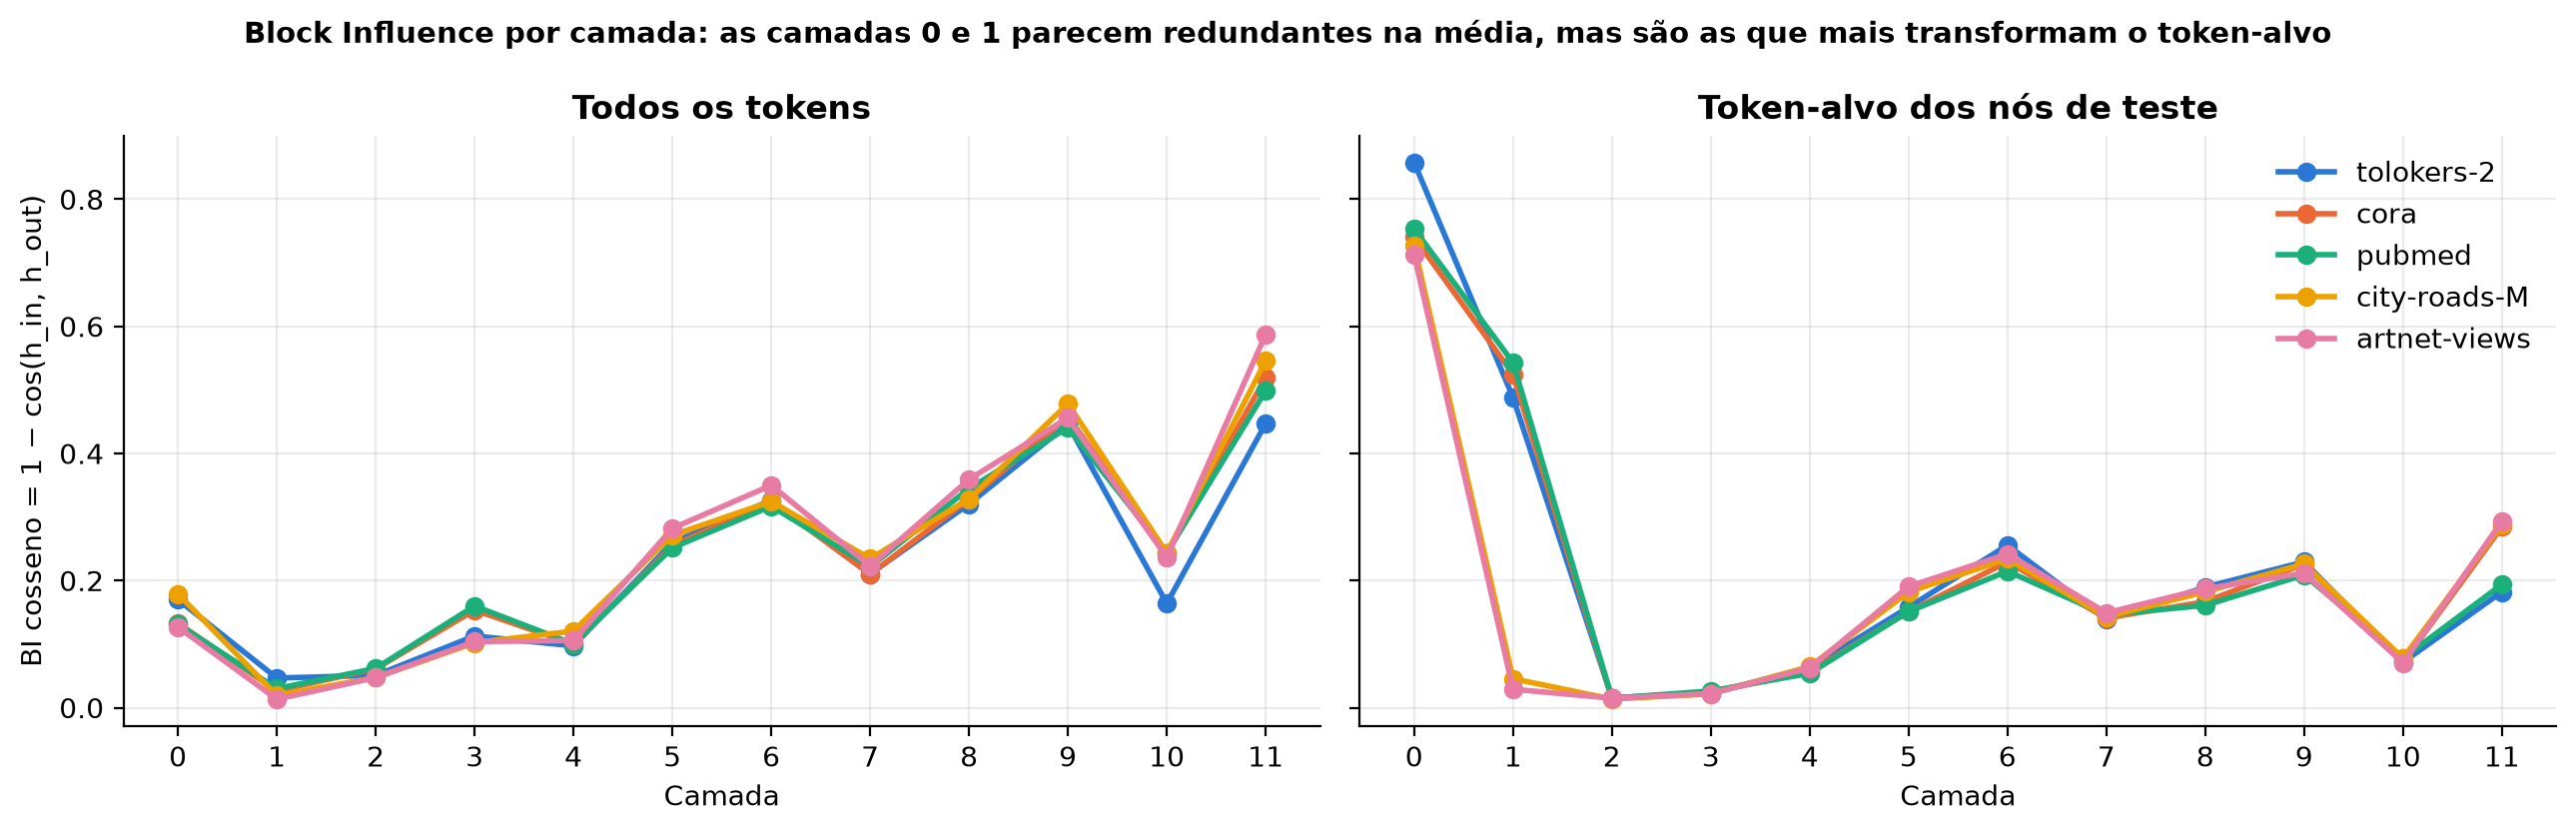
\includegraphics[width=\textwidth]{graphpfn/bi_por_camada.png}
\caption{BI por camada em cada dataset: média de todos os tokens (esquerda) e token-alvo dos nós de teste (direita).}
\label{fig:gpfn-bi}
\end{figure}

Principais observações:
\begin{itemize}
  \item \textbf{O BI é estável.} O desvio-padrão entre sementes é no máximo 0,0034. O ranking de BI é praticamente o mesmo em todos os datasets (Spearman entre 0,96 e 1,00), e cosseno e angular dão o mesmo ranking (Spearman $\geq 0{,}99$). Por isso o resto da análise usa apenas o cosseno.
  \item \textbf{As duas formas de BI discordam nas camadas 0 e 1.} Na média de todos os tokens, as camadas 0 e 1 estão entre as de menor BI. No token-alvo, a camada 0 é a que mais muda o estado (0,71 a 0,86) em todos os datasets, e a camada 1 também muda muito na classificação ($\approx 0{,}5$), mas pouco na regressão ($\approx 0{,}03$). É nessas camadas que a informação das features e do contexto rotulado chega ao token que é decodificado.
  \item \textbf{Quase toda a transformação vem do bloco LimiX.} Os adaptadores de grafo alteram muito pouco o estado: BI de 0,001 a 0,09 na atenção de grafo e de 0,001 a 0,05 no MLP de grafo, com exceção do MLP de grafo da camada 11 (0,15). Veja a Figura~\ref{fig:gpfn-subbloco}.
\end{itemize}

\begin{figure}[H]
\centering
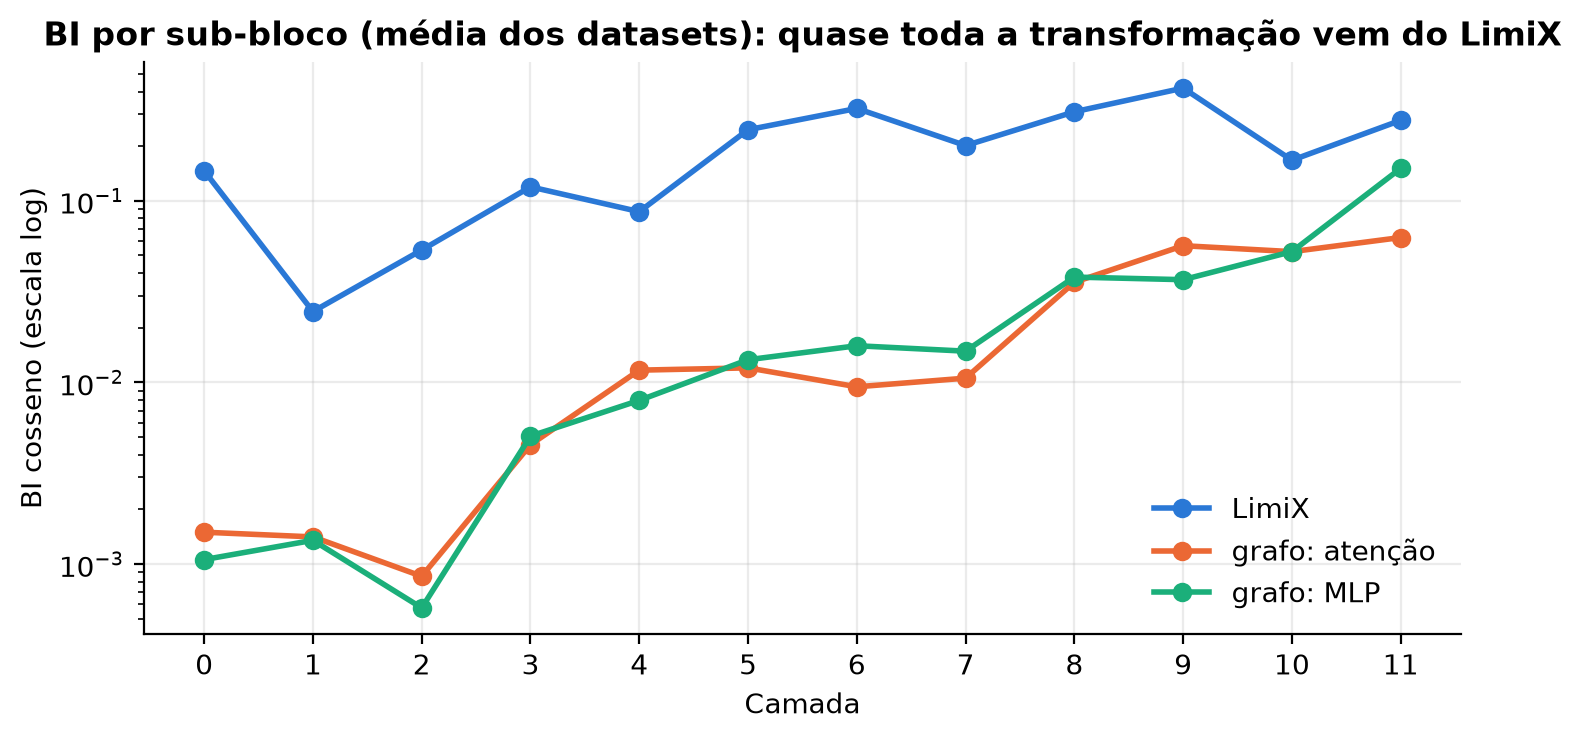
\includegraphics[width=0.8\textwidth]{graphpfn/bi_por_subbloco.png}
\caption{BI por sub-bloco (LimiX, atenção de grafo, MLP de grafo), média dos datasets, em escala logarítmica.}
\label{fig:gpfn-subbloco}
\end{figure}

\subsubsection{Ablação individual e importância real}

Cada camada foi removida sozinha, nas 3 sementes. A queda de desempenho é a importância real da camada.

\begin{table}[H]
\centering
\caption{Desempenho retido no teste (\%) ao remover \emph{uma única} camada. Em vermelho, valores abaixo de 50\%.}
\label{tab:gpfn-loo}
\setlength{\tabcolsep}{3.6pt}
\small
\begin{tabular}{@{}l*{12}{r}@{}}
\toprule
Dataset & L0 & L1 & L2 & L3 & L4 & L5 & L6 & L7 & L8 & L9 & L10 & L11 \\
\midrule
tolokers-2   & \ruim{$-3$}  & 59 & 95 & 96 & 83 & 96 & 91 & 92 & 77 & 90 & 98 & 98 \\
cora         & \ruim{0}     & 78 & 85 & 68 & 93 & 83 & \ruim{39} & \ruim{37} & \ruim{$-30$} & \ruim{$-11$} & 52 & \ruim{44} \\
pubmed       & \ruim{$-3$}  & \ruim{7} & 84 & 95 & 88 & 92 & 80 & 57 & \ruim{40} & \ruim{40} & 92 & 86 \\
city-roads-M & \ruim{$-40$} & 94 & 94 & 94 & 95 & 87 & 94 & 87 & 66 & 73 & 94 & 51 \\
artnet-views & \ruim{$-41$} & 96 & 93 & 96 & 93 & 95 & 89 & 93 & 67 & 67 & 93 & 71 \\
\bottomrule
\end{tabular}
\end{table}

\begin{itemize}
  \item \textbf{A camada 0 é indispensável}: removê-la sozinha leva todos os datasets ao nível do acaso ou abaixo ($-41\%$ a 0\%).
  \item \textbf{A camada 1 é crítica na classificação e dispensável na regressão}: retém 7\% no pubmed e 59\% no tolokers-2, mas 94--96\% nos datasets de regressão. O BI do token-alvo antecipa essa diferença; o BI de todos os tokens não.
  \item \textbf{Nenhuma camada é ``livre'' em todos os datasets.} As camadas 8 e 9 são importantes no cora e no pubmed, mas não no tolokers-2.
\end{itemize}

\begin{table}[H]
\centering
\caption{Correlação de Spearman ($\rho$) entre o BI de cada camada e sua importância real ($100 -$ retido na validação, ao remover a camada sozinha). $\rho$ positivo indica que BI alto corresponde a camada importante.}
\label{tab:gpfn-corr}
\begin{tabular}{@{}lcc@{}}
\toprule
Dataset & $\rho$ (BI de todos os tokens) & $\rho$ (BI do token-alvo) \\
\midrule
tolokers-2   & \ruim{$-0{,}27$} & 0,55 \\
cora         & 0,64  & 0,46 \\
pubmed       & 0,01  & 0,71 \\
city-roads-M & 0,62  & 0,82 \\
artnet-views & 0,66  & 0,75 \\
\midrule
Média        & 0,33  & \bom{0,66} \\
\bottomrule
\end{tabular}
\end{table}

\begin{figure}[H]
\centering
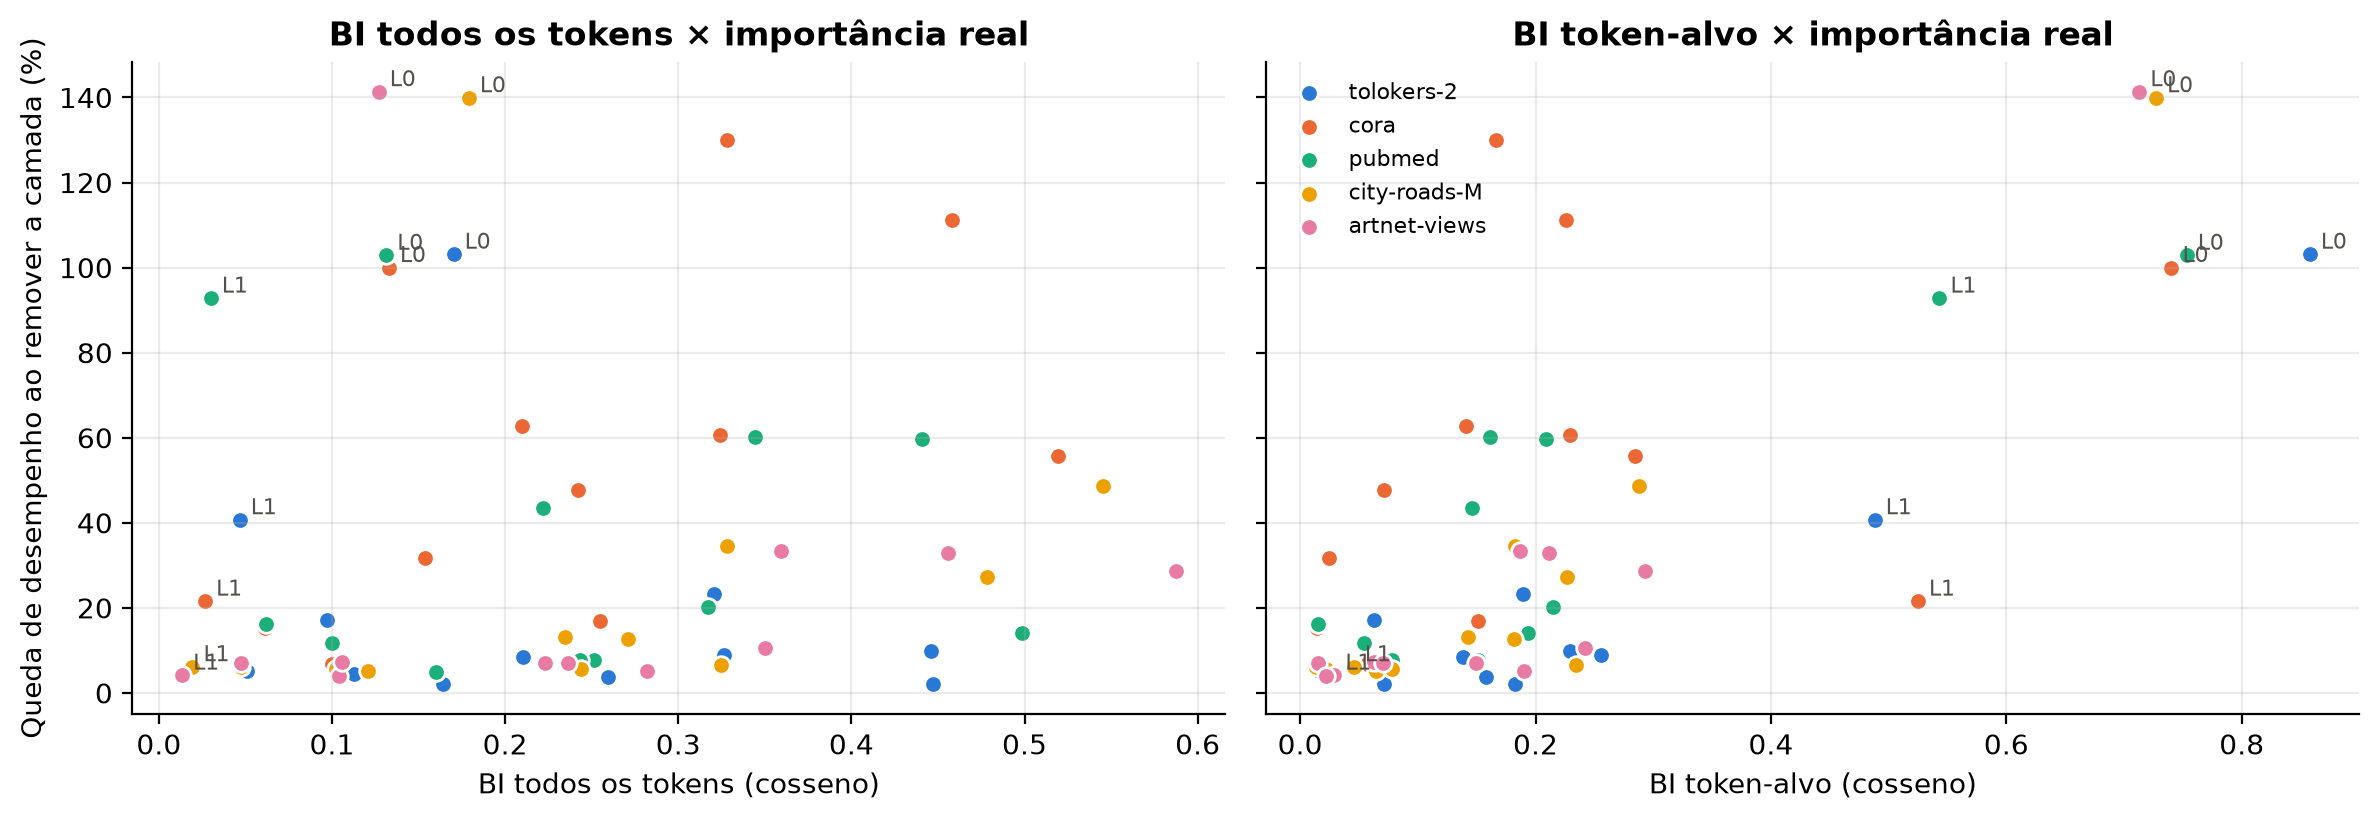
\includegraphics[width=\textwidth]{graphpfn/bi_vs_importancia.png}
\caption{BI $\times$ queda de desempenho ao remover a camada sozinha. As camadas 0 e 1 estão anotadas.}
\label{fig:gpfn-bivsimp}
\end{figure}

A correlação é fraca com o BI de todos os tokens (0,33 em média, e negativa no tolokers-2) e moderada com o BI do token-alvo (0,66).

\subsubsection{Curvas de poda}

\begin{table}[H]
\centering
\caption{Camadas removidas em cada estratégia, para $k = 1, \dots, 5$ (a poda é cumulativa).}
\label{tab:gpfn-ordens}
\small
\resizebox{\textwidth}{!}{%
\begin{tabular}{@{}llll@{}}
\toprule
Estratégia & Dataset & Ordem (primeiras 5) & Removidas com $k=5$ \\
\midrule
\multirow{3}{*}{BI de todos os tokens}
 & tolokers-2 & 1, 2, 4, 3, 10 & \{1, 2, 3, 4, 10\} \\
 & cora, pubmed & 1, 2, 4, 0, 3 & \{\ruim{0}, 1, 2, 3, 4\} \\
 & city-roads-M, artnet-views & 1, 2, 3, 4, 0 & \{\ruim{0}, 1, 2, 3, 4\} \\
\midrule
\multirow{2}{*}{BI do token-alvo}
 & tolokers-2, cora, pubmed & 2, 3, 4, 10, 7 & \{2, 3, 4, 7, 10\} \\
 & city-roads-M, artnet-views & 2, 3, 1, 4, 10 & \{1, 2, 3, 4, 10\} \\
\midrule
\multirow{5}{*}{Ablação individual (val)}
 & tolokers-2 & 11, 10, 5, 3, 2 & \{2, 3, 5, 10, 11\} \\
 & cora & 4, 2, 1, 5, 3 & \{1, 2, 3, 4, 5\} \\
 & pubmed & 5, 4, 10, 3, 2 & \{2, 3, 4, 5, 10\} \\
 & city-roads-M & 4, 3, 10, 1, 2 & \{1, 2, 3, 4, 10\} \\
 & artnet-views & 1, 3, 5, 2, 7 & \{1, 2, 3, 5, 7\} \\
\bottomrule
\end{tabular}}
\end{table}

\begin{table}[H]
\centering
\caption{Desempenho retido no teste (\%) em função do número de camadas removidas $k$ (média de 3 sementes; a linha ``Aleatória'' é a mediana das 5 ordens aleatórias). Em negrito, valores $\geq 95\%$; em vermelho, valores $\leq 0\%$ (nível do acaso ou pior).}
\label{tab:gpfn-curvas}
\small
\resizebox{\textwidth}{!}{%
\begin{tabular}{@{}llrrrrrr@{}}
\toprule
Dataset & Estratégia & $k=1$ & $k=2$ & $k=3$ & $k=4$ & $k=5$ & $k=6$ \\
\midrule
\multirow{4}{*}{tolokers-2}
 & BI todos os tokens & 59,3 & 79,5 & 64,3 & 75,2 & 44,1 & 27,2 \\
 & BI token-alvo      & 94,8 & 91,0 & 84,5 & 62,4 & 59,2 & 21,0 \\
 & Ablação (val)      & \bom{97,9} & 92,3 & 83,5 & 52,1 & 26,6 & 4,7 \\
 & Aleatória          & 90,4 & 78,7 & 53,0 & 30,3 & 21,3 & 24,3 \\
\midrule
\multirow{4}{*}{cora}
 & BI todos os tokens & 78,4 & 74,2 & 43,2 & \ruim{$-68{,}1$} & \ruim{$-48{,}2$} & \ruim{$-53{,}2$} \\
 & BI token-alvo      & 84,8 & 94,5 & 62,8 & \ruim{$-18{,}0$} & \ruim{$-56{,}8$} & \ruim{$-52{,}4$} \\
 & Ablação (val)      & 93,2 & 64,4 & 43,2 & \ruim{$-56{,}5$} & \ruim{$-49{,}1$} & \ruim{$-49{,}3$} \\
 & Aleatória          & 55,1 & \ruim{$-11{,}0$} & \ruim{$-37{,}6$} & \ruim{$-64{,}4$} & \ruim{$-53{,}4$} & \ruim{$-53{,}4$} \\
\midrule
\multirow{4}{*}{pubmed}
 & BI todos os tokens & 7,2 & 71,0 & 71,8 & \ruim{0,0} & \ruim{$-2{,}3$} & \ruim{$-77{,}5$} \\
 & BI token-alvo      & 83,9 & 90,6 & 58,4 & 50,3 & 10,1 & \ruim{$-2{,}8$} \\
 & Ablação (val)      & 92,3 & 39,8 & 55,9 & \ruim{$-1{,}3$} & 0,1 & \ruim{$-11{,}2$} \\
 & Aleatória          & 56,0 & 20,7 & \ruim{$-10{,}7$} & \ruim{$-4{,}7$} & \ruim{$-75{,}0$} & \ruim{0,0} \\
\midrule
\multirow{4}{*}{city-roads-M}
 & BI todos os tokens & 93,9 & 90,3 & 86,9 & 78,2 & \ruim{$-56{,}5$} & \ruim{$-28{,}1$} \\
 & BI token-alvo      & 93,9 & 91,0 & 86,9 & 78,2 & 72,7 & 53,4 \\
 & Ablação (val)      & 95,0 & 88,4 & 80,3 & 73,2 & 72,7 & 27,9 \\
 & Aleatória          & 93,9 & 77,0 & 58,1 & 10,5 & 4,0 & \ruim{$-0{,}9$} \\
\midrule
\multirow{4}{*}{artnet-views}
 & BI todos os tokens & \bom{95,8} & 82,6 & 84,8 & 63,1 & \ruim{$-59{,}7$} & \ruim{$-37{,}1$} \\
 & BI token-alvo      & 93,1 & 86,7 & 84,8 & 63,1 & 52,7 & 33,1 \\
 & Ablação (val)      & \bom{95,8} & 90,9 & 76,1 & 62,3 & 24,3 & 24,3 \\
 & Aleatória          & 92,8 & 68,7 & 57,5 & 16,7 & \ruim{$-1{,}5$} & \ruim{$-5{,}1$} \\
\bottomrule
\end{tabular}}
\end{table}

\begin{figure}[H]
\centering
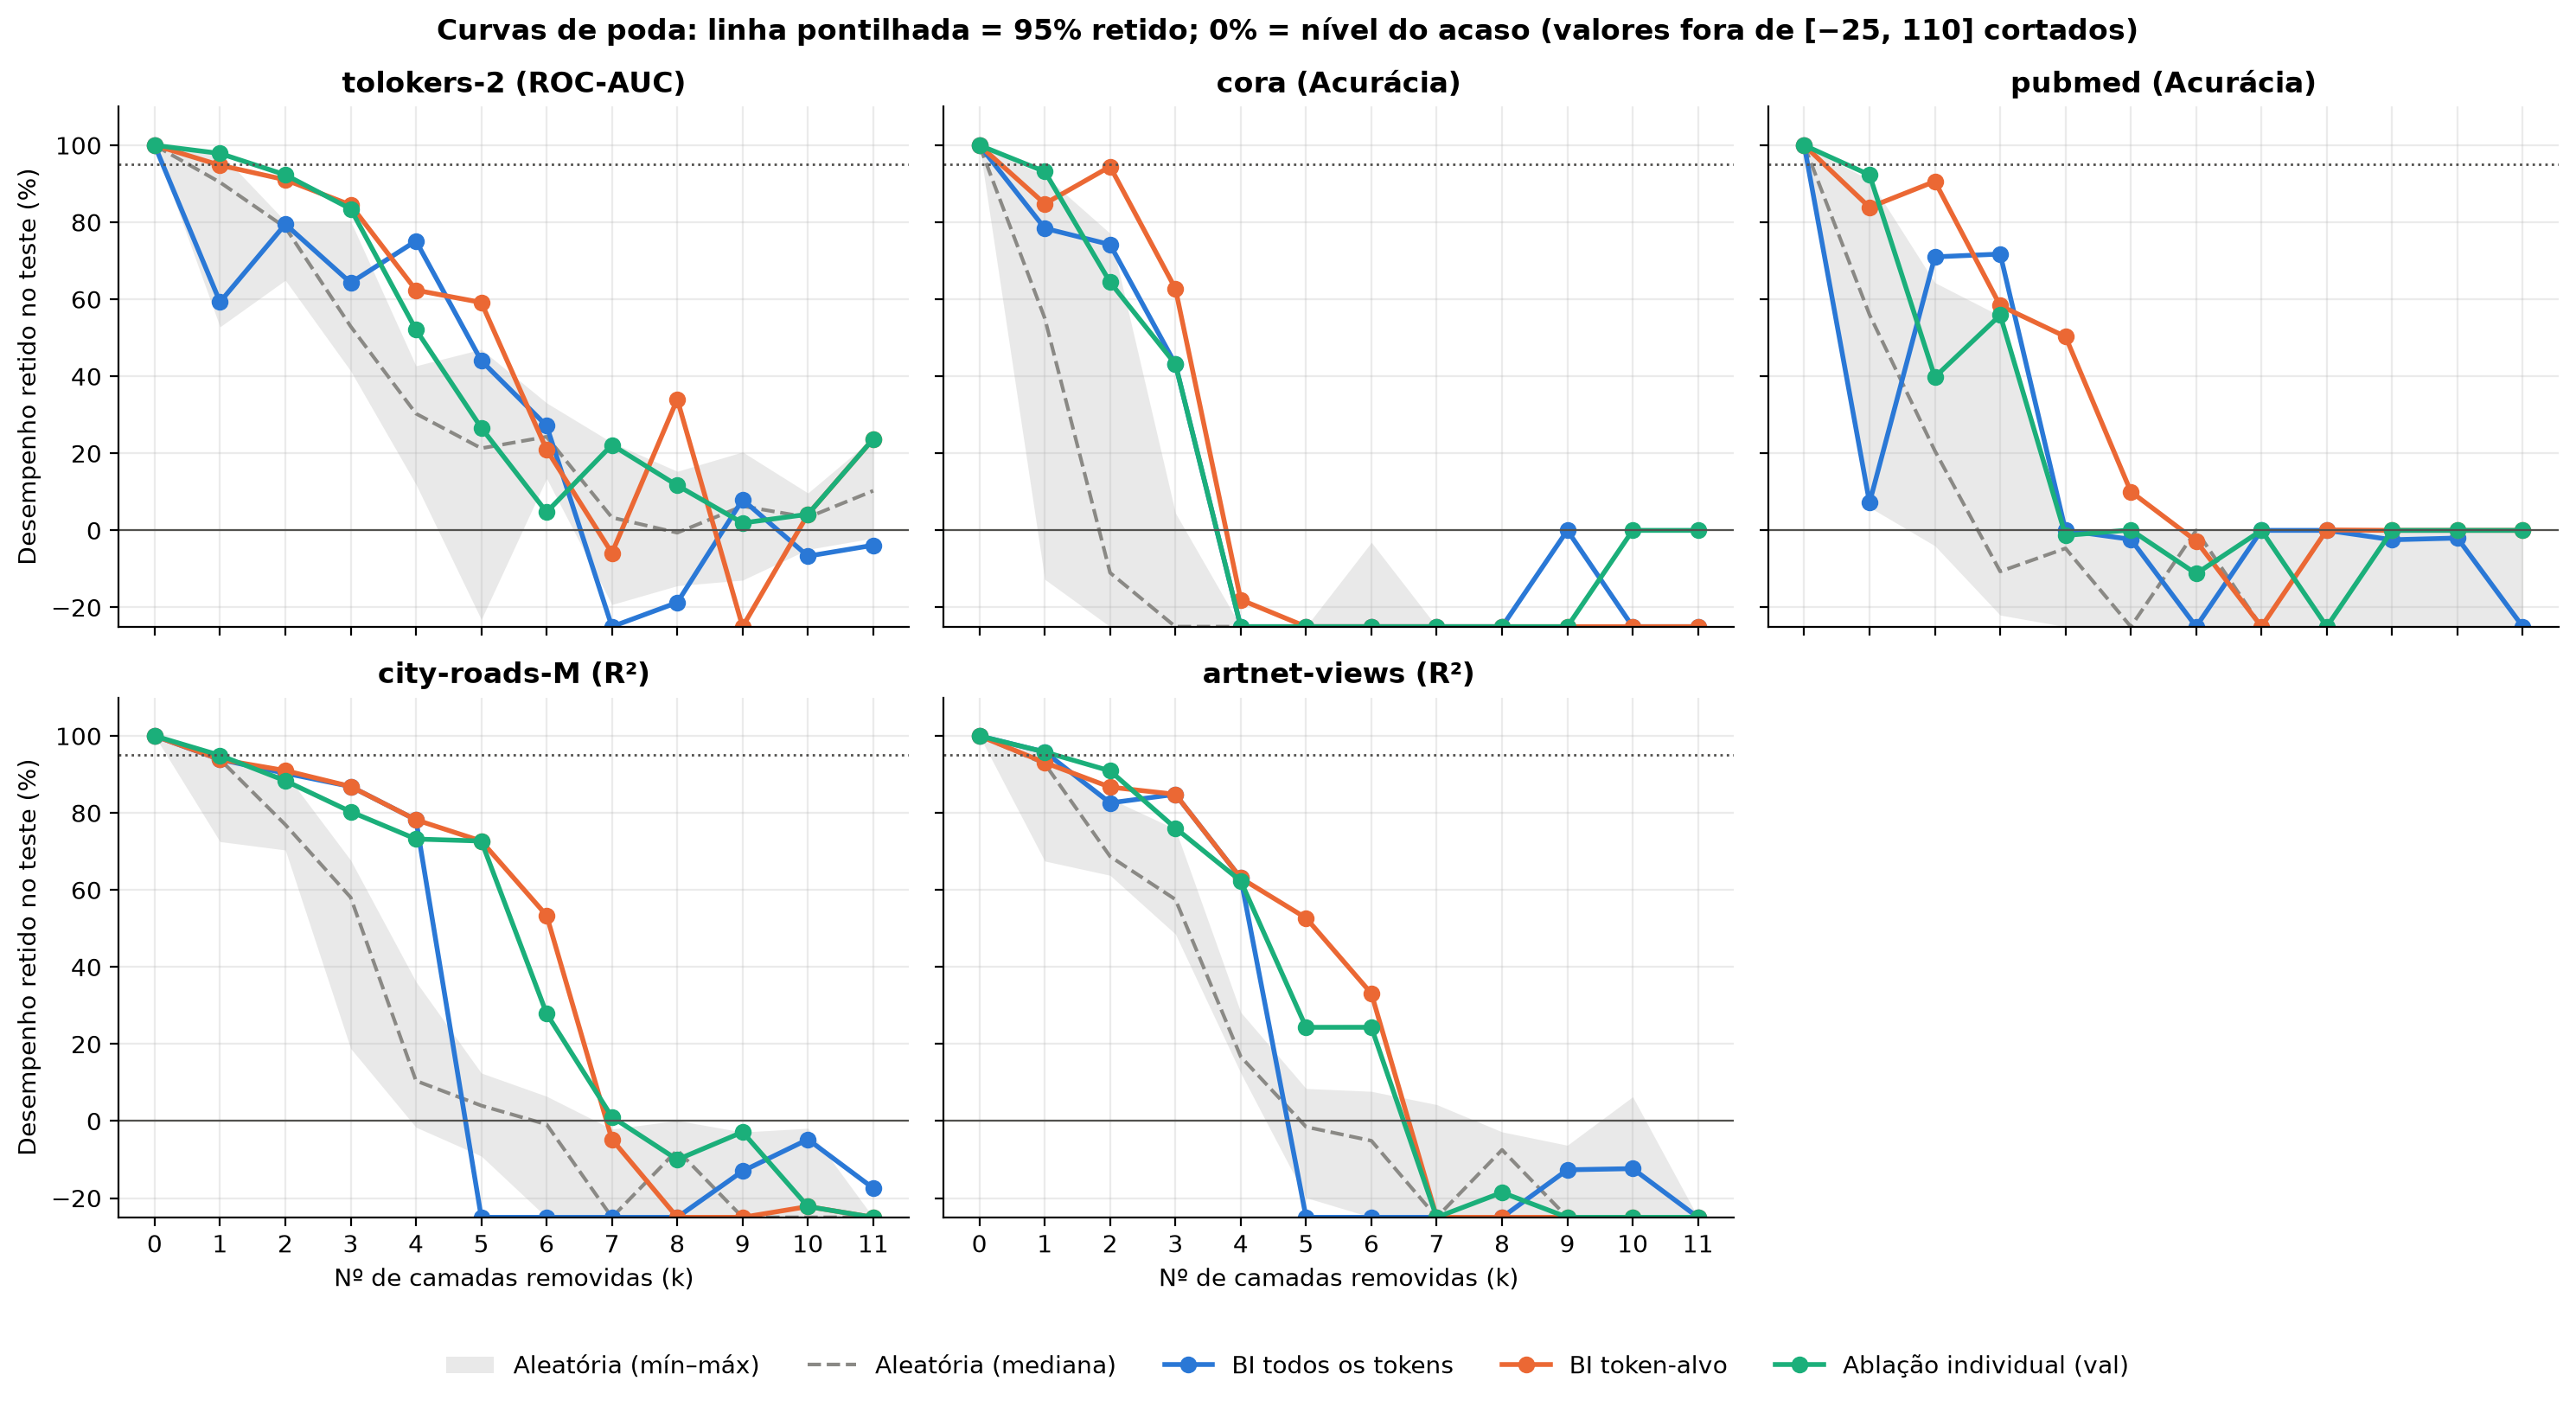
\includegraphics[width=\textwidth]{graphpfn/curvas_poda.png}
\caption{Curvas de poda. Linha pontilhada: 95\% retido. Faixa cinza: mínimo e máximo das 5 ordens aleatórias.}
\label{fig:gpfn-curvas}
\end{figure}

\begin{table}[H]
\centering
\caption{Desempenho retido médio nos 5 datasets ao remover 3 camadas.}
\label{tab:gpfn-k3}
\begin{tabular}{@{}lr@{}}
\toprule
Estratégia & Retido com $k=3$ \\
\midrule
BI do token-alvo         & \bom{75,5\%} \\
BI de todos os tokens    & 70,2\% \\
Ablação individual (val) & 67,8\% \\
Aleatória (mediana)      & 24,1\% \\
\bottomrule
\end{tabular}
\end{table}

\begin{itemize}
  \item \textbf{O BI é muito melhor que o acaso.} Com $k=3$, o BI de todos os tokens vence a ordem aleatória nos 5 datasets (70\% contra 24\% retido, em média). O BI do token-alvo é ainda melhor (75,5\%).
  \item \textbf{A perda aparece já nas primeiras camadas removidas.} Reter 95\% ou mais só acontece com $k=1$ e só em dois datasets: artnet-views (BI de todos os tokens e ablação) e tolokers-2 (ablação). Com 2 ou 3 camadas removidas, a perda já fica entre 10\% e 50\%.
  \item \textbf{O BI de todos os tokens falha justamente onde remove as camadas 0 e 1.} No pubmed, com $k=1$, ele remove a camada 1 e o desempenho retido cai para 7\%. Com $k=5$, a camada 0 entra na lista e city-roads-M e artnet-views, que vinham estáveis (78\% e 63\% com $k=4$), despencam para $-57\%$ e $-60\%$. O BI do token-alvo, que nunca remove a camada 0 nas primeiras posições, mantém 73\% e 53\% nesses mesmos pontos.
  \item \textbf{Nem a ablação evita a perda}, embora escolha as camadas olhando rótulos de validação. Isso mostra que o limite não vem de uma falha do BI: as camadas do GraphPFN não são redundantes.
\end{itemize}

\subsubsection{Custo}

\begin{table}[H]
\centering
\caption{Parâmetros e latência em função do número de camadas removidas. Latência medida no city-roads-M (57\,073 nós), mediana de 3 execuções, incluindo pré e pós-processamento.}
\label{tab:gpfn-custo}
\begin{tabular}{@{}rrrrrr@{}}
\toprule
$k$ & Camadas & Parâmetros (M) & Redução & Latência (s) & Redução \\
\midrule
0  & 12 & 20,09 & --     & 4,12 & --     \\
2  & 10 & 16,84 & 16,2\% & 3,43 & 16,8\% \\
4  & 8  & 13,59 & 32,3\% & 2,79 & 32,3\% \\
6  & 6  & 10,35 & 48,5\% & 2,14 & 48,2\% \\
8  & 4  & 7,10  & 64,7\% & 1,48 & 64,1\% \\
10 & 2  & 3,85  & 80,8\% & 0,82 & 80,1\% \\
\bottomrule
\end{tabular}
\end{table}

O ganho de custo é linear: cada camada vale cerca de 8\% dos parâmetros e 8\% da latência. A perda de desempenho cresce muito mais rápido que isso.

%------------------------------------------------------------------------------
\subsection{Variações da poda por BI}
%------------------------------------------------------------------------------

Depois da análise acima, a poda pelo BI cosseno de todos os tokens (``poda das $k$ menores'') foi repetida em duas variações, sempre sem re-treino e comparando o modelo podado com o completo nas mesmas sementes.

\subsubsection{Camada 0 protegida}

A camada 0 tem BI baixo na média de todos os tokens, mas é a única indispensável (Tabela~\ref{tab:gpfn-loo}). Na versão \emph{protegida}, as $k$ camadas de menor BI são escolhidas apenas entre as camadas 1--11. Foram usados os mesmos 5 datasets, pipeline e sementes; o PCA passou a usar semente fixa (o SVD aleatorizado do pacote fazia o baseline do cora variar cerca de $\pm 2$ p.p.; com isso, o baseline do cora é 0,668 em vez de 0,674).

\begin{table}[H]
\centering
\caption{Métrica principal no teste (média de 3 sementes), removendo as $k$ camadas de menor BI com a camada 0 protegida. Entre parênteses, a versão sem restrição, quando difere. Para $k \leq 3$ as duas versões coincidem.}
\label{tab:gpfn-protegida}
\setlength{\tabcolsep}{3pt}
\scriptsize
\begin{tabular}{@{}lccccc@{}}
\toprule
Configuração & tolokers-2 (ROC-AUC) & cora (acc.) & pubmed (acc.) & city-roads-M ($R^2$) & artnet-views ($R^2$) \\
\midrule
Completo & 0,859 & 0,668 & 0,714 & 0,640 & 0,621 \\
$k=2$ & 0,786 & 0,592 & 0,627 & 0,578 & 0,513 \\
$k=3$ & 0,731 & 0,479 & 0,629 & 0,556 & 0,527 \\
$k=4$ & 0,770 & 0,301 (\ruim{0,064}) & 0,482 (\ruim{0,413}) & 0,501 & 0,392 \\
$k=5$ & 0,658 & 0,249 (\ruim{0,155}) & 0,427 (\ruim{0,406}) & 0,407 (\ruim{$-0{,}362$}) & 0,272 (\ruim{$-0{,}371$}) \\
$k=6$ & 0,553 (0,598) & 0,147 (0,130) & 0,403 (0,180) & 0,342 (\ruim{$-0{,}180$}) & 0,206 (\ruim{$-0{,}230$}) \\
\bottomrule
\end{tabular}
\end{table}

\begin{figure}[H]
\centering
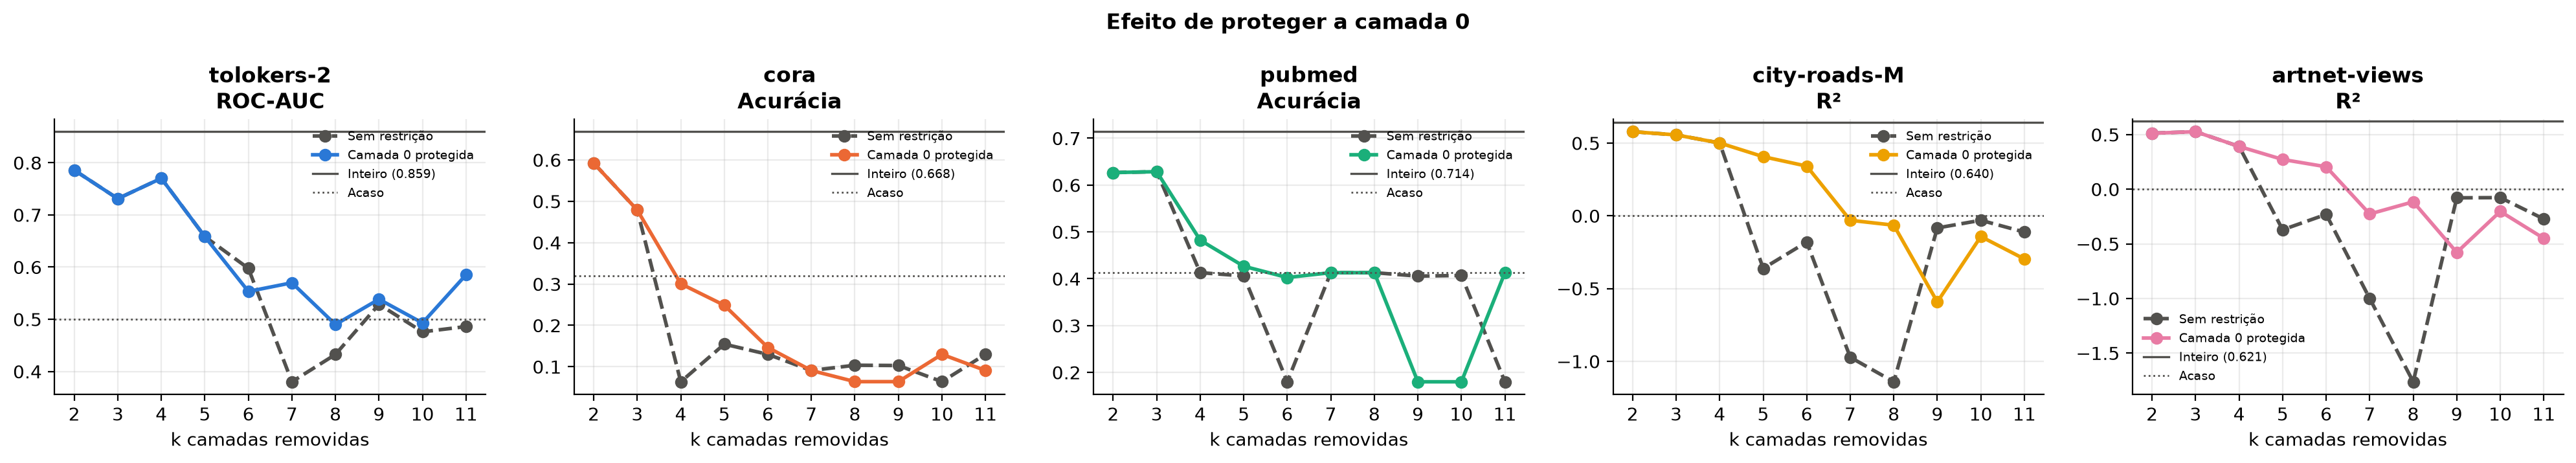
\includegraphics[width=\textwidth]{graphpfn/comparacao_livre_vs_protegida.png}
\caption{Poda das $k$ camadas de menor BI: versão livre $\times$ camada 0 protegida.}
\label{fig:gpfn-protegida}
\end{figure}

Proteger a camada 0 evita o colapso abrupto (na regressão, $R^2$ positivo até $k=6$), mas a perda continua grande e cresce a cada camada removida. Em classificação, a camada 1 passa a ser o gargalo: ela é a primeira a sair e, sozinha, já tira 7 a 9 pontos de acurácia.

\subsubsection{Protocolo e datasets do artigo}

Para comparar com os números publicados, a poda foi repetida com os datasets e o protocolo do artigo do GraphPFN (Seção 5.1 e Apêndice D): split RL do GraphLand, split aleatório 10/10/80 nos datasets clássicos, PCA de 64 dimensões só em amazon-ratings e questions, ensemble de 10 membros e 3 sementes (o artigo usa 10). Métricas: AP na classificação binária, acurácia na multiclasse e $R^2$ na regressão. A inferência foi feita em blocos para caber em 16\,GB de GPU, com resultado idêntico ao \emph{forward} original (diferença máxima de $0$ nas predições, verificado no tolokers-2).

O artigo avalia 13 datasets (Tabela 10 do artigo): 8 do benchmark GraphLand e 5 clássicos. A Tabela~\ref{tab:gpfn-datasets-artigo} lista todos e indica quais foram usados aqui. Dez foram usados; três ficaram de fora porque não couberam na GPU de 16\,GB (o artigo usou uma A100 de 80\,GB), mesmo com a inferência em blocos. O GraphPFN processa o grafo inteiro em um único \emph{forward}, como um tensor de tamanho nós $\times$ tokens (features) $\times$ 192, e a atenção nas arestas cresce com o número de arestas:
\begin{itemize}
  \item \textbf{city-reviews}: é o maior em número de nós (148\,801) e tem 2,3 milhões de arestas após a simetrização;
  \item \textbf{avazu-ctr}: tem 22 milhões de arestas após a simetrização (grau médio 288) e 229 features, o que torna os adaptadores de grafo (atenção nas arestas, por token) grandes demais;
  \item \textbf{pubmed}: tem 500 features e, seguindo o artigo, é usado \emph{sem} PCA (o artigo relata que o PCA degrada o resultado nesse dataset), o que gera 500 tokens por nó. Na análise principal (Seção anterior) o pubmed coube porque lá foi usado PCA de 64 dimensões e o split Planetoid.
\end{itemize}
Além disso, o facebook foi usado com uma diferença: a versão de 128 features do PyG é baixada de um domínio fora do ar, então foram usados o mesmo grafo e rótulos do repositório original (MUSAE), com as features reduzidas a 128 dimensões por TruncatedSVD.

\begin{table}[H]
\centering
\caption{Datasets do artigo do GraphPFN (Tabela 10 do artigo) e uso neste relatório.}
\label{tab:gpfn-datasets-artigo}
\resizebox{\textwidth}{!}{%
\begin{tabular}{@{}llrrrll@{}}
\toprule
Dataset & Coleção & Nós & Arestas & Features & Tarefa & Usado? \\
\midrule
artnet-exp     & GraphLand & 50\,405  & 280\,348     & 75  & Binária        & Sim \\
city-reviews   & GraphLand & 148\,801 & 1\,165\,415  & 37  & Binária        & \ruim{Não (sem memória)} \\
tolokers-2     & GraphLand & 11\,758  & 519\,000     & 16  & Binária        & Sim \\
artnet-views   & GraphLand & 50\,405  & 280\,348     & 50  & Regressão      & Sim \\
avazu-ctr      & GraphLand & 76\,269  & 10\,984\,077 & 260 & Regressão      & \ruim{Não (sem memória)} \\
city-roads-M   & GraphLand & 57\,073  & 107\,104     & 26  & Regressão      & Sim \\
hm-prices      & GraphLand & 46\,563  & 10\,730\,995 & 41  & Regressão      & Sim \\
twitch-views   & GraphLand & 168\,114 & 6\,797\,557  & 4   & Regressão      & Sim \\
amazon-ratings & Clássico  & 24\,492  & 93\,050      & 300 & Multiclasse (5)  & Sim (PCA 64) \\
facebook       & Clássico  & 22\,470  & 170\,823     & 128 & Multiclasse (4)  & Sim (SVD) \\
pubmed         & Clássico  & 19\,717  & 44\,324      & 500 & Multiclasse (3)  & \ruim{Não (sem memória)} \\
questions      & Clássico  & 48\,921  & 153\,540     & 301 & Binária        & Sim (PCA 64) \\
wiki-cs        & Clássico  & 11\,701  & 215\,603     & 300 & Multiclasse (10) & Sim \\
\bottomrule
\end{tabular}}
\end{table}

\noindent Arestas e features conforme a Tabela 10 do artigo (arestas não direcionadas, antes da simetrização). Na análise principal, o cora não faz parte do artigo; foi incluído como dataset clássico pequeno de referência.

\begin{table}[H]
\centering
\caption{Modelo completo: reprodução do artigo (métrica no teste).}
\label{tab:gpfn-reproducao}
\begin{tabular}{@{}llcc@{}}
\toprule
Dataset & Métrica & Completo (aqui) & Artigo (ICL) \\
\midrule
artnet-exp     & AP       & 0,519 & 0,518 \\
tolokers-2     & AP       & 0,613 & 0,613 \\
artnet-views   & $R^2$    & 0,629 & 0,628 \\
city-roads-M   & $R^2$    & 0,649 & 0,649 \\
hm-prices      & $R^2$    & 0,780 & 0,779 \\
twitch-views   & $R^2$    & 0,733 & 0,732 \\
amazon-ratings & Acurácia & 0,439 & 0,449 \\
facebook       & Acurácia & 0,911 & 0,924 \\
questions      & AP       & 0,208 & 0,214 \\
wiki-cs        & Acurácia & 0,821 & 0,820 \\
\bottomrule
\end{tabular}
\end{table}

O modelo completo reproduz o artigo: nos 6 datasets do GraphLand e no wiki-cs, os valores batem até a 3ª casa. As diferenças em amazon-ratings, facebook e questions ($\leq 0{,}013$) vêm do sorteio do split 10/10/80 e, no facebook, das features reconstruídas por SVD. No protocolo do artigo, o ranking de BI também é praticamente o mesmo nos 10 datasets: as camadas 1 e 2 sempre têm o menor BI, seguidas de 3 e 4, e a camada 0 aparece entre a 4ª e a 6ª posições.

\begin{table}[H]
\centering
\caption{Métrica do artigo no teste, média de 3 sementes. ``Protegida'' = camada 0 nunca removida.}
\label{tab:gpfn-artigo}
\setlength{\tabcolsep}{2.2pt}
\scriptsize
\resizebox{\textwidth}{!}{%
\begin{tabular}{@{}lcccccccccc@{}}
\toprule
Configuração & artnet-exp & tolokers-2 & artnet-views & city-roads-M & hm-prices & twitch-views & amazon-r. & facebook & questions & wiki-cs \\
\midrule
Completo & 0,519 & 0,612 & 0,629 & 0,649 & 0,780 & 0,733 & 0,439 & 0,911 & 0,208 & 0,821 \\
$k=2$ (camadas 1 e 2) & 0,318 & 0,522 & 0,528 & 0,596 & 0,652 & 0,643 & 0,354 & 0,778 & 0,078 & 0,774 \\
$k=3$ & 0,368 & 0,415 & 0,529 & 0,566 & 0,403 & 0,446 & 0,392 & 0,757 & 0,059 & 0,633 \\
$k=4$, livre & 0,197 & 0,459 & 0,378 & 0,519 & 0,394 & 0,209 & \ruim{0,067} & \ruim{0,243} & 0,032 & \ruim{0,067} \\
$k=4$, protegida & 0,197 & 0,459 & 0,378 & 0,519 & 0,394 & 0,209 & 0,386 & 0,737 & 0,060 & 0,608 \\
$k=5$, livre & 0,103 & 0,345 & \ruim{$-0{,}409$} & \ruim{$-0{,}514$} & \ruim{$-0{,}446$} & 0,120 & 0,279 & 0,284 & 0,028 & 0,107 \\
$k=5$, protegida & 0,134 & 0,345 & 0,250 & 0,453 & 0,195 & 0,120 & 0,380 & 0,598 & 0,049 & 0,449 \\
$k=6$, protegida & 0,110 & 0,338 & 0,194 & 0,425 & 0,041 & 0,059 & 0,363 & 0,408 & 0,042 & 0,239 \\
\midrule
\emph{Acaso} & \emph{0,100} & \emph{0,218} & \emph{0} & \emph{0} & \emph{0} & \emph{0} & \emph{0,369} & \emph{0,306} & \emph{0,030} & \emph{0,230} \\
\bottomrule
\end{tabular}}
\end{table}

\begin{figure}[H]
\centering
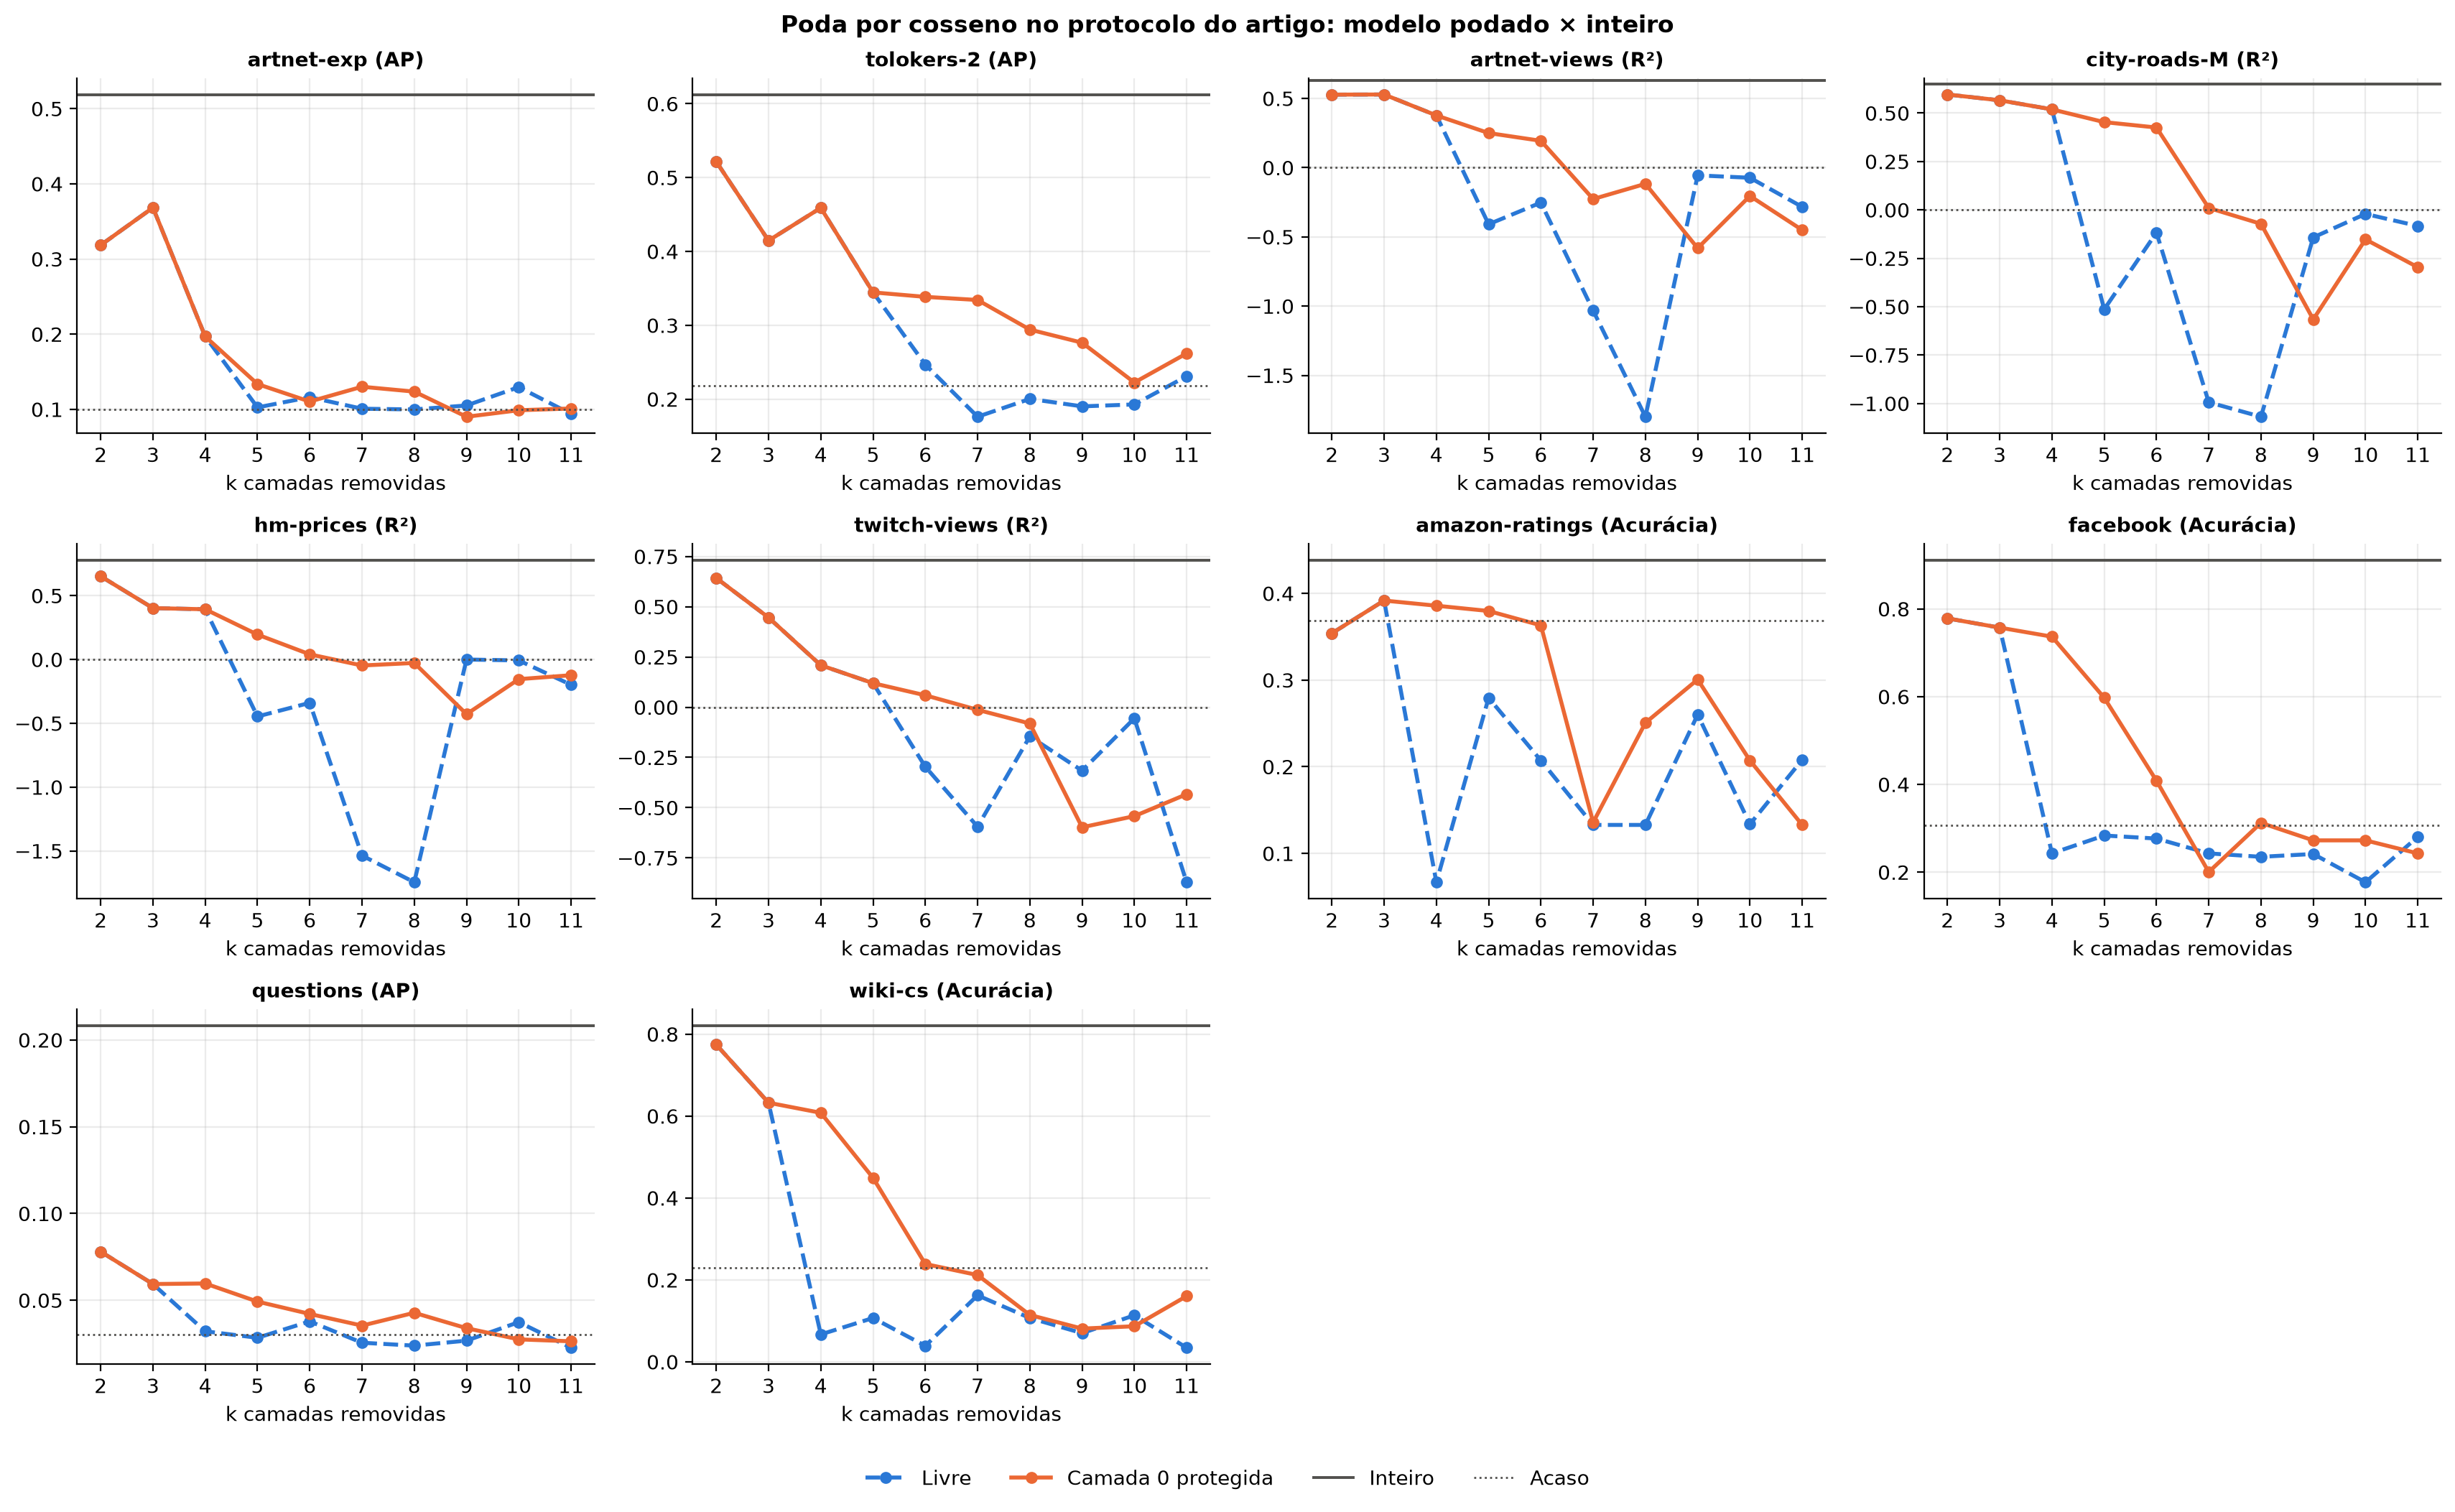
\includegraphics[width=\textwidth]{graphpfn/metrica_artigo_todos.png}
\caption{Poda por BI no protocolo do artigo: métrica no teste em função de $k$, versões livre e com a camada 0 protegida.}
\label{fig:gpfn-artigo}
\end{figure}

O padrão se repete no protocolo do artigo: removendo só as camadas 1 e 2 ($-16\%$ dos parâmetros), a queda vai de 0,05 (city-roads-M, wiki-cs) a 0,20 (artnet-exp), e o amazon-ratings já fica abaixo do acaso. Na versão livre, o modelo colapsa quando a camada 0 entra na lista ($k=4$ nos datasets clássicos, $k=5$ na regressão). Com a camada 0 protegida, o colapso é evitado, mas não a perda.

%------------------------------------------------------------------------------
\subsection{Conclusões sobre o BI}
%------------------------------------------------------------------------------

\textbf{Remover camadas inteiras do GraphPFN escolhidas por Block Influence, sem re-treino, causa perda de desempenho já a partir de duas camadas.} Ao contrário dos LLMs, em que o ShortGPT encontra camadas quase redundantes, as 12 camadas do LimiX-16M são todas usadas.

\begin{itemize}
  \item O BI ajuda a ordenar as camadas (é muito melhor que o acaso), mas a ordem não basta: mesmo a ordem quase ótima, escolhida por ablação com rótulos de validação, perde mais de 5\% a partir de 2 camadas.
  \item O BI calculado como média sobre todos os tokens é enganoso neste modelo, porque os tokens de feature dominam a média e escondem que as camadas 0 e 1 são as que mais alteram o token-alvo. Para modelos que decodificam apenas parte dos tokens, o BI deve ser medido nesses tokens.
  \item Os adaptadores de grafo alteram muito pouco o estado (BI até 0,09, exceto o MLP de grafo da camada 11) e representam 18\% dos parâmetros de cada camada.
\end{itemize}

\paragraph{Fontes.}
{\raggedright \path{GraphFPN/analise_camadas_e_poda_graphpfn.ipynb}, \path{GraphFPN/poda_cosseno_k_menores_sem_camada0_graphpfn.ipynb} e \path{GraphFPN/poda_cosseno_artigo_graphpfn.ipynb}; CSVs em \path{Block_Influence_results/graphfpn_analise_unificada/}, \path{graphfpn_poda_cosseno_k_sem_camada0/} e \path{graphfpn_poda_cosseno_artigo/}.\par}

%==============================================================================
\section{G2T-FM e NodePFN, comparados ao GraphPFN}
\label{sec:pfns}
%==============================================================================

Esta seção repete a análise do GraphPFN em dois outros PFNs para grafos, para saber se o comportamento visto lá é geral: \textbf{BI por camada, poda sem re-treino, KD e custo}. Para que a comparação seja direta, o próprio GraphPFN foi reavaliado no mesmo protocolo (mesmos datasets, splits, ensemble de 10 e ordens de poda); as linhas ``GraphPFN'' das tabelas abaixo vêm dessa reavaliação, e não da análise principal da Seção anterior (que usa splits Planetoid e 1 membro de ensemble).

\subsection{Os modelos}

\begin{itemize}
  \item \textbf{G2T-FM (G2T-LimiX):} é o mesmo LimiX-16M do GraphPFN, mas \emph{sem} adaptadores de grafo. A estrutura do grafo entra como features extras (agregações de vizinhos e PEARL, de pesos fixos). São 12 camadas e 16,53\,M parâmetros, com ICL e ensemble de 10 membros. Como o modelo é o mesmo do GraphPFN sem os adaptadores, a comparação mostra se o padrão de BI vem do LimiX ou dos adaptadores.
  \item \textbf{NodePFN:} é um PFN de grafo pré-treinado do zero, um Transformer de 12 camadas (29,01\,M parâmetros). Cada nó é um único token, com features suavizadas pelo grafo e reduzidas por TSVD. Funciona só em ICL.
\end{itemize}

\subsection{Metodologia}

O protocolo é o do artigo do GraphPFN (Tabela~\ref{tab:gpfn-datasets-artigo}): split RL no GraphLand, split aleatório 10/10/80 nos clássicos e 3 sementes. Os datasets são tolokers-2, amazon-ratings e wiki-cs nos três modelos, mais city-roads-M no GraphPFN e no G2T-LimiX (o NodePFN não faz regressão). As etapas são as mesmas do GraphPFN:
\begin{enumerate}
  \item reproduzir o modelo inteiro;
  \item medir o BI (todos os tokens e token-alvo; no NodePFN as duas formas coincidem, porque cada nó é um token) e a ablação individual de cada camada;
  \item podar $k=1\ldots6$ camadas sem re-treino, pelas ordens BI de todos os tokens, BI do token-alvo, ablação (referência; usa rótulos) e 3 permutações aleatórias, sempre com a camada 0 protegida;
  \item KD com 6 camadas removidas ($\approx-50\%$ dos parâmetros), comparando um student inicializado pelo modelo podado com um de mesma arquitetura e pesos aleatórios, no mesmo protocolo do KD do GraphPFN.
\end{enumerate}
Desempenho retido, como no GraphPFN: $100\cdot(s_{\text{podado}}-s_{\text{acaso}})/(s_{\text{inteiro}}-s_{\text{acaso}})$.

\subsection{Resultados}

\subsubsection{Modelo inteiro}

\begin{table}[H]
\centering
\caption{Modelo inteiro no teste, média de 3 sementes, e referência publicada.}
\label{tab:novos-inteiro}
\begin{tabular}{@{}llcc@{}}
\toprule
Modelo & Dataset (métrica) & Aqui & Referência \\
\midrule
G2T-LimiX & tolokers-2 (AP)           & 0,618 & 0,616 \\
G2T-LimiX & city-roads-M ($R^2$)      & 0,651 & 0,652 \\
G2T-LimiX & amazon-ratings (acurácia) & 0,445 & 0,450 \\
G2T-LimiX & wiki-cs (acurácia)        & 0,813 & 0,809 \\
\midrule
NodePFN   & tolokers-2 (AP)           & 0,415 $\pm$ 0,029 & 0,438 \\
NodePFN   & amazon-ratings (acurácia) & 0,399 $\pm$ 0,003 & 0,412 \\
NodePFN   & wiki-cs (acurácia)        & 0,786 $\pm$ 0,001 & 0,781 \\
\bottomrule
\end{tabular}
\end{table}

\noindent Referências: artigo do G2T-FM (Tabelas 2 e 3) e artigo do GraphPFN (Tabela 11, para o NodePFN). O G2T-LimiX reproduz o artigo com diferenças de $-0{,}005$ a $+0{,}004$. O NodePFN fica $0{,}023$ abaixo no tolokers-2 e varia muito entre sementes ($\pm 0{,}029$), com causa não identificada. No amazon-ratings, os dois modelos ficam só 0,03--0,08 acima do acaso (0,369), o que torna o desempenho retido instável nesse dataset.

\subsubsection{Block Influence e ablação individual}

\begin{table}[H]
\centering
\caption{Desempenho retido no teste (\%) ao remover uma única camada, média de 3 sementes.}
\label{tab:novos-loo}
\setlength{\tabcolsep}{3pt}
\resizebox{\textwidth}{!}{%
\begin{tabular}{@{}llrrrrrrrrrrrr@{}}
\toprule
Modelo & Dataset & L0 & L1 & L2 & L3 & L4 & L5 & L6 & L7 & L8 & L9 & L10 & L11 \\
\midrule
GraphPFN & tolokers-2     & \ruim{12}   & \ruim{44} & 93 & 91 & 81 & 93 & 86 & 86 & 75 & 77 & 96 & 96 \\
GraphPFN & wiki-cs        & \ruim{$-20$} & 91 & 97 & 97 & 97 & 90 & 90 & 90 & 70 & 56 & 94 & 81 \\
GraphPFN & city-roads-M   & \ruim{$-72$} & 95 & 95 & 94 & 95 & 89 & 93 & 86 & 65 & 73 & 94 & 53 \\
GraphPFN & amazon-ratings & \ruim{$-270$} & $-22$ & 60 & 70 & 55 & 73 & 88 & 93 & $-1$ & 39 & 85 & 83 \\
\midrule
G2T-LimiX & tolokers-2     & \ruim{6}    & 99 & 98 & 99 & 98 & 95 & 93 & 93 & 41 & 81 & 97 & 98 \\
G2T-LimiX & wiki-cs        & \ruim{$-17$} & 94 & 97 & 98 & 98 & 97 & 99 & 89 & 73 & 68 & 97 & 87 \\
G2T-LimiX & city-roads-M   & \ruim{$-3$}  & 99 & 95 & 96 & 94 & 94 & 93 & 89 & 60 & 86 & 95 & 87 \\
G2T-LimiX & amazon-ratings & \ruim{$-317$} & 85 & 56 & 58 & 56 & 76 & 70 & 67 & $-2$ & 23 & 90 & 71 \\
\midrule
NodePFN & tolokers-2     & \ruim{$-26$}  & 106 & 78 & 86 & 97 & 88 & 112 & 106 & 98 & 108 & 104 & 105 \\
NodePFN & wiki-cs        & \ruim{$-8$}   & 101 & 74 & 45 & 74 & 95 & 96 & 98 & 98 & 98 & 96 & 99 \\
NodePFN & amazon-ratings & \ruim{$-343$} & 116 & $-18$ & $-70$ & 5 & 94 & 90 & 76 & 101 & 88 & 87 & $-7$ \\
\bottomrule
\end{tabular}}
\end{table}

\begin{table}[H]
\centering
\caption{Ordem de poda pelo BI cosseno (5 primeiras camadas) e correlação de Spearman entre BI e importância real (validação).}
\label{tab:novos-bi}
\resizebox{\textwidth}{!}{%
\begin{tabular}{@{}llllcc@{}}
\toprule
Modelo & Dataset & Ordem (todos os tokens) & Ordem (token-alvo) & $\rho$ todos & $\rho$ alvo \\
\midrule
GraphPFN & tolokers-2     & 1, 2, 4, 3, 10 & 2, 3, 4, 10, 7 & $-0{,}10$ & 0,62 \\
GraphPFN & wiki-cs        & 1, 2, 4, \ruim{0}, 3 & 2, 3, 4, 10, 7 & 0,48 & 0,78 \\
GraphPFN & city-roads-M   & 1, 2, 3, 4, \ruim{0} & 2, 3, 1, 4, 10 & 0,69 & 0,80 \\
GraphPFN & amazon-ratings & 1, 2, 4, \ruim{0}, 3 & 2, 3, 4, 10, 7 & $-0{,}37$ & 0,29 \\
\midrule
G2T-LimiX & tolokers-2     & 1, 2, 4, \ruim{0}, 3 & 2, 3, 4, 10, 11 & 0,52 & 0,80 \\
G2T-LimiX & wiki-cs        & 1, 2, \ruim{0}, 4, 3 & 3, 2, 4, 10, 5 & 0,25 & 0,71 \\
G2T-LimiX & city-roads-M   & 1, 2, 4, 3, \ruim{0} & 2, 3, 4, 1, 10 & 0,62 & 0,82 \\
G2T-LimiX & amazon-ratings & 1, 2, 4, \ruim{0}, 3 & 2, 3, 4, 10, 7 & $-0{,}06$ & 0,08 \\
\midrule
NodePFN & tolokers-2     & \multicolumn{2}{c}{9, 11, 8, 5, 10} & \multicolumn{2}{c}{0,42} \\
NodePFN & wiki-cs        & \multicolumn{2}{c}{9, 11, 7, 5, 8}  & \multicolumn{2}{c}{0,54} \\
NodePFN & amazon-ratings & \multicolumn{2}{c}{9, 10, 11, 5, 8} & \multicolumn{2}{c}{0,37} \\
\bottomrule
\end{tabular}}
\end{table}

\begin{itemize}
  \item \textbf{GraphPFN no protocolo comum:} o padrão da análise principal se confirma. A camada 0 é indispensável e, no tolokers-2, também a 1 (44\%); o BI do token-alvo acompanha a importância ($\rho$ = 0,62--0,80 nos três datasets informativos), e o de todos os tokens não ($-0{,}10$ a 0,69).
  \item \textbf{No G2T-LimiX o padrão do GraphPFN se repete.} As camadas 1 e 2 têm o menor BI na média de todos os tokens, e a camada 0 aparece entre as 5 primeiras. Mas a camada 0 é indispensável e é a que mais muda o token-alvo (BI do alvo 0,72--0,85). O BI do token-alvo acompanha a importância real muito melhor ($\rho$ = 0,71--0,82, contra 0,25--0,62). Como o G2T-LimiX não tem adaptadores de grafo, esse padrão vem do LimiX.
  \item \textbf{No NodePFN o padrão é outro.} As camadas de menor BI são as finais (9, 11, 10, 8), e a correlação com a importância é moderada (0,37--0,54). Também aqui a camada 0 é a única indispensável em todos os datasets.
  \item \textbf{Cosseno e angular concordam.} Nos 7 casos (G2T-LimiX e NodePFN), o ranking do BI cosseno e do BI angular tem Spearman $\geq 0{,}979$ e as 6 camadas removidas no KD são as mesmas. Por isso as ordens usam só o cosseno, como no GraphPFN e no AnyGraph.
  \item Em ambos, as camadas críticas além da 0 mudam com o dataset: camada 8 no G2T-LimiX; camadas 2--4 no NodePFN.
\end{itemize}

\subsubsection{Poda sem re-treino}

\begin{table}[H]
\centering
\caption{Desempenho retido no teste (\%) ao remover as $k$ primeiras camadas de cada ordem (camada 0 protegida), média de 3 sementes. Aleatória = mediana de 3 ordens. amazon-ratings omitido (modelo inteiro perto do acaso).}
\label{tab:novos-curvas}
\resizebox{\textwidth}{!}{%
\begin{tabular}{@{}lllrrrrrr@{}}
\toprule
Modelo & Dataset & Ordem & $k=1$ & $k=2$ & $k=3$ & $k=4$ & $k=5$ & $k=6$ \\
\midrule
\multirow{4}{*}{GraphPFN} & \multirow{4}{*}{tolokers-2}
  & BI todos  & \ruim{44} & 77 & 50 & 61 & 32 & 31 \\
 & & BI alvo  & 93 & 81 & 67 & 42 & 49 & 21 \\
 & & ablação  & 96 & 82 & 63 & 41 & 22 & 15 \\
 & & aleatória & 91 & 61 & 57 & 47 & 20 & 12 \\
\midrule
\multirow{4}{*}{GraphPFN} & \multirow{4}{*}{wiki-cs}
  & BI todos  & 91 & 92 & 68 & 64 & 37 & 1 \\
 & & BI alvo  & 97 & 94 & 82 & 59 & 20 & $-1$ \\
 & & ablação  & 97 & 88 & 82 & 59 & 2 & $-10$ \\
 & & aleatória & 90 & 65 & 6 & 9 & $-13$ & $-31$ \\
\midrule
\multirow{4}{*}{GraphPFN} & \multirow{4}{*}{city-roads-M}
  & BI todos  & 95 & 92 & 87 & 80 & 70 & 66 \\
 & & BI alvo  & 95 & 92 & 87 & 80 & 75 & 66 \\
 & & ablação  & 95 & 88 & 80 & 80 & 46 & 37 \\
 & & aleatória & 93 & 66 & 67 & 39 & 25 & 1 \\
\midrule
\multirow{4}{*}{G2T-LimiX} & \multirow{4}{*}{tolokers-2}
  & BI todos  & 99 & 96 & 75 & 64 & 46 & 42 \\
 & & BI alvo  & 98 & 97 & 85 & 65 & 55 & 33 \\
 & & ablação  & 99 & 97 & 93 & 65 & 38 & 20 \\
 & & aleatória & 95 & 58 & 54 & 46 & 38 & 25 \\
\midrule
\multirow{4}{*}{G2T-LimiX} & \multirow{4}{*}{wiki-cs}
  & BI todos  & 94 & 97 & 77 & 59 & 3 & 1 \\
 & & BI alvo  & 98 & 94 & 81 & 48 & $-3$ & $-8$ \\
 & & ablação  & 98 & 94 & 49 & 10 & $-10$ & $-13$ \\
 & & aleatória & 98 & 70 & 25 & $-3$ & $-6$ & $-16$ \\
\midrule
\multirow{4}{*}{G2T-LimiX} & \multirow{4}{*}{city-roads-M}
  & BI todos  & 99 & 89 & 79 & 71 & 39 & 32 \\
 & & BI alvo  & 95 & 87 & 73 & 71 & 36 & 32 \\
 & & ablação  & 99 & 92 & 84 & 67 & 36 & 35 \\
 & & aleatória & 94 & 78 & 28 & 32 & $-41$ & 29 \\
\midrule
\multirow{3}{*}{NodePFN} & \multirow{3}{*}{wiki-cs}
  & BI (todos = alvo) & 98 & 98 & 95 & 89 & 84 & 78 \\
 & & ablação  & 101 & 99 & 97 & 94 & 90 & 84 \\
 & & aleatória & 95 & 83 & 79 & 41 & 41 & 27 \\
\midrule
\multirow{3}{*}{NodePFN} & \multirow{3}{*}{tolokers-2}
  & BI (todos = alvo) & 108 & 106 & 110 & 109 & 110 & 109 \\
 & & ablação  & 108 & 112 & 118 & 117 & 115 & 109 \\
 & & aleatória & 88 & 89 & 102 & 105 & 109 & 114 \\
\bottomrule
\end{tabular}}
\end{table}

\begin{itemize}
  \item \textbf{GraphPFN no protocolo comum:} com $k=3$, o BI do token-alvo retém 67\% (tolokers-2), 82\% (wiki-cs) e 87\% (city-roads-M), contra 57\%, 6\% e 67\% da ordem aleatória, e empata com a ablação ou a supera. O BI de todos os tokens remove a camada 1 primeiro e, no tolokers-2, onde ela é crítica, perde 56 pontos já com $k=1$. No city-roads-M a poda é a mais tolerante dos PFNs no LimiX: 66\% com 6 camadas removidas.
  \item \textbf{G2T-LimiX:} como no GraphPFN, só 1 ou 2 camadas saem sem perda grande. Com $k=3$, o BI do token-alvo retém 85\% (tolokers-2), 81\% (wiki-cs) e 73\% (city-roads-M), contra 54\%, 25\% e 28\% da ordem aleatória. O GraphPFN, no mesmo ponto, retém 67\%, 82\% e 87\% no protocolo comum (75,5\% na análise principal).
  \item \textbf{NodePFN:} é o modelo mais tolerante à poda. No wiki-cs, retém 95\% com 3 camadas removidas e 78\% com 6. No tolokers-2, todas as ordens passam de 100\%, inclusive as aleatórias. Isso indica que o modelo inteiro está abaixo do seu potencial nesse dataset (ele já ficava abaixo da referência), e não que a poda ajude.
  \item \textbf{amazon-ratings:} nos dois modelos, o retido oscila entre $+116\%$ e $-184\%$ porque o modelo inteiro está muito perto do acaso. Já com $k=3$, as ordens por BI ficam perto do acaso ou abaixo dele.
\end{itemize}

\subsubsection{KD com 6 camadas removidas}

O student podado mantém as 6 camadas de maior BI (com a camada 0): no G2T-LimiX, as camadas 0, 5, 6, 8, 9 e 11 (16,53\,M $\to$ 8,56\,M, $-48\%$); no NodePFN, as camadas 0--4 e 6, ou 0--4 e 10 no wiki-cs (29,01\,M $\to$ 14,80\,M, $-49\%$).

\begin{table}[H]
\centering
\caption{KD com 6 camadas removidas, nos três PFNs: desempenho retido no teste (\%, normalizado pelo acaso como na poda), média de 3 sementes, antes e depois do KD. Entre parênteses, o \% do professor (student $\div$ professor) usado no EXP-004.}
\label{tab:novos-kd}
\resizebox{\textwidth}{!}{%
\begin{tabular}{@{}llc|rr|rr@{}}
\toprule
 & & & \multicolumn{2}{c|}{Student podado} & \multicolumn{2}{c}{Student aleatório} \\
Modelo & Dataset (métrica) & Professor & antes & depois & antes & depois \\
\midrule
GraphPFN  & tolokers-2 (AP)          & 0,612 & 32  & \bom{94} (95,8) & 6 & 14 (44,8) \\
GraphPFN  & city-roads-M ($R^2$)     & 0,649 & 66  & \bom{96} (96,2) & $-24$ & 15 (15,1) \\
GraphPFN  & wiki-cs (acurácia)       & \multicolumn{5}{c}{não cabe em 16\,GB (ver Seção~\ref{sec:limitacoes})} \\
GraphPFN  & amazon-ratings (acurácia) & 0,439 & $-9$ & 58 (93,3) & $-279$ & $-238$ (46,3) \\
\midrule
G2T-LimiX & tolokers-2 (AP)          & 0,617 & 44  & \bom{91} (94,5) & 8 & 30 (54,6) \\
G2T-LimiX & city-roads-M ($R^2$)     & 0,651 & 32  & \bom{91} (90,7) & $-25$ & 0 (0,0) \\
G2T-LimiX & wiki-cs (acurácia)       & 0,812 & 1   & \ruim{33} (52,2) & $-21$ & $-20$ (13,6) \\
G2T-LimiX & \quad sem parada antecipada$^\ddagger$ & 0,813 & $-6$ & \bom{95} (96,4) & $-20$ & $-3$ (26,3) \\
G2T-LimiX & amazon-ratings (acurácia)$^\dagger$ & 0,445 & $-90$ & \ruim{$-7$} (81,6) & $-95$ & $-99$ (65,9) \\
\midrule
NodePFN   & tolokers-2 (AP)          & 0,415 & 109 & \bom{107} (103,3) & 6 & 73 (86,7) \\
NodePFN   & wiki-cs (acurácia)       & 0,786 & 78  & \bom{99} (99,3) & $-22$ & $-18$ (16,2) \\
NodePFN   & amazon-ratings (acurácia) & 0,399 & $-157$ & 33 (94,7) & $-527$ & $-516$ (53,2) \\
\bottomrule
\end{tabular}}
\end{table}

\noindent $^\dagger$ Contexto de treino limitado a 900 nós por passo para caber em 16\,GB (desvio de protocolo). $^\ddagger$ Sensibilidade: 200 passos sem parada antecipada, mesmo lr das execuções originais; podado nas 2 sementes que tinham travado (0 e 1), aleatório nas 3 sementes.

\begin{itemize}
  \item \textbf{A normalização importa.} O ``\% do professor'' esconde falhas: no amazon-ratings, 81--95\% do professor correspondem a um retido de $-7$ a 58\%, porque o professor está só 0,03--0,07 acima do acaso. Por isso a tabela usa o retido, como na poda; o amazon-ratings não é informativo para o KD em nenhum dos três modelos.
  \item \textbf{O podado recupera, o aleatório não.} Nos 6 casos informativos (tolokers-2, city-roads-M e wiki-cs, excluindo o GraphPFN no wiki-cs e o NodePFN no tolokers-2), o student podado volta a 91--99\% de retido depois do KD em 5; a exceção é o G2T-LimiX no wiki-cs (33\% no protocolo principal; ver abaixo). O student aleatório, com o mesmo orçamento, fica entre $-20$ e 30\%; no city-roads-M ele converge para uma saída constante ($R^2 \approx 0$).
  \item \textbf{A falha do G2T-LimiX no wiki-cs era da parada antecipada.} Nas sementes 0 e 1, o student podado passa por um platô com saída quase constante e a paciência de 4 avaliações encerrava o treino ali. Sem parada antecipada, as duas chegam a 0,784 (95\% de retido), igual à semente 2 do protocolo principal (0,783). O student aleatório continua no acaso mesmo sem parada antecipada.
  \item \textbf{A vantagem do podado depende do orçamento de treino.} No GraphPFN (tolokers-2, semente 0), o student aleatório treinado por 1\,000 passos sem parada chega a 82\% de retido, contra 14\% com o protocolo principal. A conclusão correta é que o student podado recupera \emph{muito mais rápido} (menos de 200 passos), não que o aleatório nunca recupere.
  \item \textbf{No NodePFN o KD quase não é necessário no tolokers-2,} porque o podado já supera o professor antes do treino. No wiki-cs, o KD leva o podado de 78\% para 99\%.
\end{itemize}

\subsubsection{Custo da poda}

O custo foi medido do mesmo jeito nos três PFNs: tolokers-2, semente 0, pipeline completo de avaliação (pré-processamento, ensemble de 10 e inferência em blocos), $k = 0, 2, 4, 6$ camadas removidas pela ordem do BI de todos os tokens (camada 0 protegida). A latência é a mediana de 3 execuções depois de 1 de aquecimento. O AnyGraph foi medido no arxiv (Seção~\ref{sec:any-fases}).

\begin{table}[H]
\centering
\caption{Custo por número de camadas removidas: parâmetros (M), latência de uma avaliação completa (s) e pico de memória da GPU (GB). Entre parênteses, a variação em relação ao modelo inteiro.}
\label{tab:custo}
\resizebox{\textwidth}{!}{%
\begin{tabular}{@{}llrrrr@{}}
\toprule
Modelo (dataset) & Medida & $k=0$ & $k=2$ & $k=4$ & $k=6$ \\
\midrule
\multirow{3}{*}{GraphPFN (tolokers-2)} & Parâmetros & 20,09 & 16,84 & 13,59 & 10,35 ($-48\%$) \\
 & Latência & 12,9 & 10,8 & 8,8 & 6,7 ($-48\%$) \\
 & Pico GPU & 0,94 & 0,93 & 0,93 & 0,92 ($-2\%$) \\
\midrule
\multirow{3}{*}{G2T-LimiX (tolokers-2)} & Parâmetros & 16,53 & 13,87 & 11,22 & 8,56 ($-48\%$) \\
 & Latência & 22,1 & 19,1 & 16,2 & 13,4 ($-39\%$) \\
 & Pico GPU & 4,17 & 4,16 & 4,15 & 4,14 ($-1\%$) \\
\midrule
\multirow{3}{*}{NodePFN (tolokers-2)} & Parâmetros & 29,01 & 24,27 & 19,54 & 14,80 ($-49\%$) \\
 & Latência & 2,50 & 2,20 & 1,91 & 1,62 ($-35\%$) \\
 & Pico GPU & 4,30 & 4,30 & 4,30 & 4,30 ($0\%$) \\
\midrule
\multirow{2}{*}{AnyGraph link2 (arxiv)} & Parâmetros & 16,88 & 12,66 & 8,44 & 4,22 ($-75\%$) \\
 & Latência & 1,49 & 1,43 & 1,36 & 1,31 ($-12\%$) \\
\bottomrule
\end{tabular}}
\end{table}

\begin{itemize}
  \item \textbf{Nos PFNs, a latência cai quase na proporção das camadas:} $-35$ a $-48\%$ com 6 de 12 camadas removidas. A parte que não cai é o pré-processamento (features de grafo e PEARL no G2T-LimiX, TSVD no NodePFN).
  \item \textbf{O pico de memória não muda.} Ele é dado pelas ativações de uma camada (com a inferência em blocos) e pelos dados, não pelos pesos (20\,M parâmetros ocupam menos de 0,1\,GB). Podar camadas não deixa os PFNs caberem em GPUs menores.
  \item \textbf{No AnyGraph, a poda reduz muito os parâmetros e quase nada o tempo,} porque o tempo é dominado pelos projetores e pela propagação no grafo.
\end{itemize}

\noindent O código e os resultados desta seção estão no branch \path{worktree-fase1-novos-gfms} (commits \texttt{e7e680b} e \texttt{7bd308b}, mais os scripts da rodada de 12/11 ainda não commitados), ainda fora do \texttt{main}.

\section{Síntese entre modelos}
\label{sec:sintese}

A Tabela~\ref{tab:sintese} reúne os modelos avaliados no protocolo comum. Para os PFNs (12 camadas), ``25\%'' e ``50\%'' da profundidade correspondem a $k=3$ e $k=6$; para o AnyGraph (8 camadas), a $k=2$ e $k=4$. Os valores são médias dos datasets informativos: tolokers-2, wiki-cs e city-roads-M nos PFNs (só wiki-cs no NodePFN, cujo tolokers-2 passa de 100\% com qualquer poda) e os 5 datasets no AnyGraph (link2).

\begin{table}[H]
\centering
\caption{Síntese: retido (\%) pela melhor ordem de BI (token-alvo nos PFNs) e pela ordem aleatória (mediana), correlação BI $\times$ importância, KD com $\approx$50\% dos parâmetros e redução de latência com 50\% das camadas.}
\label{tab:sintese}
\resizebox{\textwidth}{!}{%
\begin{tabular}{@{}lcccccccc@{}}
\toprule
 & \multicolumn{2}{c}{25\% removido} & \multicolumn{2}{c}{50\% removido} & & \multicolumn{2}{c}{KD (retido após)} & \\
Modelo & BI & aleatória & BI & aleatória & $\rho$ BI & podado & aleatório & Latência \\
\midrule
GraphPFN       & 79 & 43 & 29 & $-6$ & 0,73 & 95 & 15 & $-48\%$ \\
G2T-LimiX      & 80 & 36 & 19 & 13 & 0,78 & 72$^*$ & 3 & $-39\%$ \\
NodePFN (wiki-cs) & 95 & 79 & 78 & 27 & 0,53 & 99 & $-18$ & $-35\%$ \\
AnyGraph link2 & 106 & 106 & 90 & 97 & $-0{,}31$ & 96 & 115 & $-9\%$ \\
\bottomrule
\end{tabular}}
\end{table}

\noindent $^*$ Protocolo principal, como nas demais células: 91 (tolokers-2), 91 (city-roads-M) e 33 (wiki-cs). Na sensibilidade sem parada antecipada, o wiki-cs chega a 95\% e a média a 92\%; esse valor não entra na tabela porque a sensibilidade foi rodada depois de ver o resultado e só nas sementes do podado que tinham travado (Seção~\ref{sec:pfns}). OpenGraph e Prodigy (só Tiers 1 e 2) não entram na tabela: no OpenGraph, remover 1 ou 2 das 4 camadas mantém ou melhora o desempenho; no Prodigy, remover a camada de menor BI do bloco de dados não muda nada, mas remover também a do bloco de tarefa derruba o modelo ao acaso.

\begin{itemize}
  \item \textbf{Nos PFNs, o BI do token-alvo é uma boa ordem de poda:} retém o dobro da ordem aleatória com 25\% das camadas removidas e se aproxima da ordem de referência por ablação, sem usar rótulos. Com 50\% removido, nenhum PFN do LimiX (GraphPFN e G2T-LimiX) aguenta sem re-treino; o NodePFN é o mais tolerante.
  \item \textbf{No AnyGraph, o BI não ajuda,} porque quase nenhuma camada importa: as ordens aleatórias são tão boas quanto o BI e a correlação é negativa. O que determina o desempenho é o roteamento e os projetores (controle identidade).
  \item \textbf{O KD recupera $\approx$50\% de poda em todos os modelos} (95--99\% de retido no GraphPFN e no NodePFN, 72\% no G2T-LimiX por causa do wiki-cs, 96\% no AnyGraph). Nos PFNs, começar do modelo podado é essencial com orçamento curto; no AnyGraph, não é.
  \item \textbf{O ganho de custo é sobretudo de latência e de parâmetros, não de memória:} a latência dos PFNs cai 35--48\% e o pico de GPU não muda.
\end{itemize}

\subsection{Datasets em comum entre os modelos}
\label{sec:sobreposicao}

Cada modelo foi avaliado nos datasets que o seu próprio artigo ou código usa, e por isso a sobreposição entre eles é pequena (Tabela~\ref{tab:sobreposicao}).

\begin{table}[H]
\centering
\caption{Datasets usados em cada modelo. ``Plan.'' = versão Planetoid; ``própria'' = versão distribuída com o código do modelo.}
\label{tab:sobreposicao}
\resizebox{\textwidth}{!}{%
\begin{tabular}{@{}lcccccc@{}}
\toprule
Dataset & AnyGraph & OpenGraph & Prodigy & GraphPFN & G2T-LimiX & NodePFN \\
\midrule
cora           & própria & própria & & Plan.$^a$ & & \\
pubmed         & própria & própria & & Plan.$^a$ & & \\
tolokers-2     & & & & \checkmark & \checkmark & \checkmark \\
wiki-cs        & & & & \checkmark & \checkmark & \checkmark \\
amazon-ratings & & & & \checkmark & \checkmark & \checkmark \\
city-roads-M   & & & & \checkmark & \checkmark & ---$^b$ \\
artnet-views   & & & & \checkmark & & \\
outros 5 do artigo$^c$ & & & & \checkmark & & \\
arxiv, home, tech & \checkmark & & & & & \\
citeseer       & & \checkmark & & & & \\
5 de \emph{link prediction}$^d$ & & \checkmark & & & & \\
FB15k-237      & & & \checkmark & & & \\
\bottomrule
\end{tabular}}
\end{table}

\noindent $^a$ Só na análise principal do GraphPFN. $^b$ O NodePFN não faz regressão. $^c$ artnet-exp, hm-prices, twitch-views, facebook e questions (protocolo do artigo do GraphPFN). $^d$ ml1m, ml10m, collab, ddi e amazon-book.

\begin{itemize}
  \item \textbf{Nenhum dataset é comum aos seis modelos.}
  \item \textbf{Os PFNs compartilham um bloco comum:} tolokers-2, wiki-cs e amazon-ratings nos três, e city-roads-M no GraphPFN e no G2T-LimiX. É o único conjunto montado para comparação direta (mesmos splits, ensemble e ordens de poda) e é dele que vêm os números da Tabela~\ref{tab:sintese}. O amazon-ratings fica perto do acaso nos três modelos e não sustenta conclusões.
  \item \textbf{cora e pubmed aparecem em AnyGraph, OpenGraph e GraphPFN, mas não são o mesmo dado.} O cora do AnyGraph tem 25\,191 nós e 71 classes; o cora Planetoid usado no GraphPFN tem 2\,708 nós e 7 classes. O pubmed tem tamanho quase igual nas duas versões (19\,720 e 19\,717 nós), mas os splits são diferentes (teste do AnyGraph e Planetoid) e o GraphPFN aplica PCA de 64 dimensões. O OpenGraph usa os arquivos distribuídos com o próprio código.
  \item \textbf{Prodigy e o \emph{link prediction} do OpenGraph não têm dataset em comum com nenhum outro modelo.}
\end{itemize}

Por isso, a comparação numérica entre modelos vale apenas entre os PFNs. O AnyGraph entra na Tabela~\ref{tab:sintese} com os seus próprios datasets: a comparação com os PFNs é de padrão de comportamento (quanto o BI supera a ordem aleatória, quanto o KD recupera), e não de valores no mesmo dataset.

\section{Limitações}
\label{sec:limitacoes}

\begin{itemize}
  \item \textbf{Sementes.} Os PFNs usam 3 sementes (o artigo do GraphPFN usa 10) e o AnyGraph, 10 repetições pareadas. Diferenças de poucos pontos de retido entre ordens, num mesmo $k$, não são significativas.
  \item \textbf{Datasets pouco informativos.} No amazon-ratings os três PFNs ficam só 0,03--0,07 acima do acaso, e o retido oscila de forma errática. No tolokers-2, o NodePFN está abaixo da referência e quase todas as podas ``melhoram'' o modelo. Esses casos aparecem nas tabelas, mas não sustentam conclusões.
  \item \textbf{Adaptações para 16\,GB de GPU.} A inferência dos PFNs é feita em blocos (resultado idêntico ao \emph{forward} original). No KD do G2T-LimiX no amazon-ratings, o contexto de treino foi limitado a 900 nós por passo. O KD do GraphPFN no wiki-cs não coube em memória (o contexto já tem cerca de 880 nós e limitar ainda mais não resolve) e ficou de fora.
  \item \textbf{Validação no AnyGraph.} Como o AnyGraph é zero-shot e não tem validação, os nós de teste foram divididos ao meio: a ordem por ablação é escolhida numa metade e reportada na outra. Além disso, o AnyGraph não é determinístico entre execuções na GPU, por isso cada comparação usa o baseline da mesma execução.
  \item \textbf{Cenário transdutivo.} Todos os modelos rodam sobre o grafo inteiro: features e arestas dos nós de validação e de teste entram no \emph{forward} (sem rótulos), como nos pipelines oficiais. O BI que escolhe as camadas removidas também é medido em todos os nós, e a redução de dimensão das features (PCA no GraphPFN, TruncatedSVD no NodePFN) é ajustada em todos os nós. Nenhum rótulo de validação ou de teste é usado na poda nem na perda do KD; a validação escolhe a ordem por ablação, o lr e o melhor ponto do KD, e o teste só é reportado.
  \item \textbf{Mesmo split entre sementes.} O split RL do GraphLand é fixo e o 10/10/80 dos datasets clássicos foi sorteado uma vez (semente 0). As 3 sementes variam a aleatoriedade do modelo e do treino (membros do ensemble, lotes do KD, inicialização do student aleatório), não a divisão dos dados, então o desvio entre sementes não inclui a variação do split.
  \item \textbf{Sensibilidade do KD fora do protocolo principal.} A execução sem parada antecipada do G2T-LimiX no wiki-cs foi feita depois de ver o resultado, e o student podado só foi repetido nas 2 sementes que tinham travado. Ela aparece como sensibilidade (Tabela~\ref{tab:novos-kd}); a Tabela~\ref{tab:sintese} usa só o protocolo principal.
  \item \textbf{Orçamento do KD.} O protocolo principal tem até 200 passos com parada antecipada. A comparação entre student podado e aleatório depende desse orçamento: com 1\,000 passos, o aleatório do GraphPFN chega a 82\% de retido no tolokers-2 (1 semente).
  \item \textbf{Dois protocolos no GraphPFN.} A análise principal do GraphPFN (Seção anterior) usa splits Planetoid e 1 membro de ensemble; só as linhas ``GraphPFN'' da Seção~\ref{sec:pfns} estão no protocolo comum aos PFNs. As comparações entre modelos usam apenas estas.
  \item \textbf{OpenGraph e Prodigy} foram avaliados só com os Tiers 1 e 2 (sem ablação, ordens aleatórias, KD ou custo) e não entram nas comparações quantitativas.
\end{itemize}

\section{Conclusão}

As três perguntas da Introdução têm respostas diferentes conforme a família de modelo.

\begin{enumerate}
  \item \textbf{O BI encontra camadas redundantes?} Nos PFNs, sim, desde que medido no token que o modelo usa para predizer: o BI do token-alvo tem correlação de 0,53--0,82 com a importância real nos datasets informativos e retém o dobro da ordem aleatória. O BI de todos os tokens, que é a forma usual do ShortGPT, é enganado pelos tokens de feature e chega a escolher primeiro camadas críticas (a camada 0 e, no GraphPFN, a 1). No AnyGraph, o BI não é melhor que o acaso, porque as MLPs dos experts quase não contribuem.
  \item \textbf{Quanto se pode podar sem re-treino?} Pouco nos PFNs do LimiX: 1 a 2 de 12 camadas com perda pequena e cerca de 80\% retido com 3. O NodePFN aguenta mais (78\% com 6 camadas no wiki-cs). No AnyGraph, até 6 de 8 camadas, mas por motivos que não são de redundância aprendida: o modelo funciona quase só com os projetores. A poda reduz a latência dos PFNs na proporção das camadas e não reduz o pico de memória.
  \item \textbf{O KD recupera o modelo podado?} Sim: com cerca de metade dos parâmetros, o student podado volta a 91--99\% de retido nos PFNs, em menos de 200 passos, em 5 dos 6 casos informativos; no G2T-LimiX no wiki-cs, a parada antecipada encerra o treino num platô (33\%), e sem ela o podado chega a 95\%. Um student de pesos aleatórios não chega perto com o mesmo orçamento, mas recupera boa parte com 5 vezes mais passos, então o papel da poda é tornar o KD rápido e estável. No AnyGraph, um student aleatório já funciona sem treino.
\end{enumerate}

Em resumo, poda por BI do token-alvo seguida de um KD curto é uma forma barata de obter PFNs para grafos com metade dos parâmetros e cerca de 40\% menos latência, quase sem perda nos datasets em que o modelo inteiro é bem melhor que o acaso.


\begin{thebibliography}{9}
\bibitem{shortgpt} X. Men, M. Xu, Q. Zhang, B. Wang, H. Lin, Y. Lu, X. Han, W. Chen. \emph{ShortGPT: Layers in Large Language Models are More Redundant Than You Expect}. arXiv:2403.03853, 2024.
\bibitem{anygraph} L. Xia, C. Huang. \emph{AnyGraph: Graph Foundation Model in the Wild}. arXiv:2408.10700, 2024.
\bibitem{opengraph} L. Xia, B. Kao, C. Huang. \emph{OpenGraph: Towards Open Graph Foundation Models}. arXiv:2403.01121, 2024.
\bibitem{prodigy} Q. Huang, H. Ren, P. Chen, G. Kržmanc, D. Zeng, P. Liang, J. Leskovec. \emph{PRODIGY: Enabling In-context Learning Over Graphs}. NeurIPS, 2023.
\bibitem{graphpfn} D. Eremeev, O. Platonov, G. Bazhenov, A. Babenko, L. Prokhorenkova. \emph{GraphPFN: A Prior-Data Fitted Graph Foundation Model}. arXiv:2509.21489, 2025.
\bibitem{g2tfm} \emph{Turning Tabular Foundation Models into Graph Foundation Models} (G2T-FM). arXiv:2508.20906, 2025. % TODO conferir autores
\bibitem{nodepfn} J. Choi, J. Kim, W. Kang, N. Park. \emph{Learning Posterior Predictive Distributions for Node Classification from Synthetic Graph Priors} (NodePFN). ICLR, 2026.
\bibitem{hinton-kd} G. Hinton, O. Vinyals, J. Dean. \emph{Distilling the Knowledge in a Neural Network}. arXiv:1503.02531, 2015.
% TODO: adicionar LimiX e GraphLand com os dados conferidos nos artigos.
\end{thebibliography}

\end{document}
